\documentclass[hidelinks,11pt]{article}

\usepackage[utf8]{inputenc}

\usepackage{parskip,textgreek,amsmath,graphicx,hyperref,bookmark,caption,subcaption,relsize,float,array,csvsimple,pgffor,eso-pic,xcolor,titling}

\usepackage[nottoc,numbib]{tocbibind}

\usepackage[overlay,absolute]{textpos}

\usepackage[toc,page]{appendix}

\usepackage[british]{babel}
\usepackage[useregional]{datetime2}
\DTMlangsetup[en-GB]{showdayofmonth=false}

\graphicspath{{/Users/janek/PycharmProjects/BirchesScandinavia/results/}{images/}}

\setlength{\jot}{1.5ex}

\captionsetup{width=0.8\linewidth}

% set standard width of figures
\setkeys{Gin}{width=0.85\linewidth}

\setlength\tabcolsep{10pt}
\setlength\parindent{0pt}

\usepackage[margin=1.75in]{geometry}

% define abbreviations
\newcommand{\dadi}{\textdelta a\textdelta i}
\newcommand{\pendula}{\textit{B. pendula}}
\newcommand{\pubescens}{\textit{B. pubescens}}
\newcommand{\nana}{\textit{B. nana}}
\newcommand{\incana}{\textit{A. incana}}
\newcommand{\glutinosa}{\textit{A. glutinosa}}

\usepackage[acronym,toc]{glossaries}

\makeglossaries

\newacronym{sfs}{SFS}{Site-Frequency Spectrum}
\newacronym{dfe}{DFE}{Distribution of Fitness Effects}
\newacronym{snp}{SNP}{Single-Nucleotide Polymorphism}
\newacronym{lgm}{LGM}{Last Glacial Maximum}
\newacronym{mle}{MLE}{Maximum Likelihood Estimation}
\newacronym{bca}{BCa}{Bias-Corrected and accelerated}
\newacronym{hwe}{HWE}{Hardy-Weinberg Equilibrium}
\newacronym{lrt}{LRT}{Likelihood-Ratio Test}
\newacronym{bfgs}{BFGS}{Broyden-Fletcher-Goldfarb-Shanno}
\newacronym{gim}{GIM}{Godambe Information Matrix}
\newacronym{pca}{PCA}{Principal Component Analysis}
\newacronym{umap}{UMAP}{Uniform Manifold Approximation and Projection}
\newacronym{feems}{FEEMS}{Fast Estimation of Effective Migration Surfaces}
\newacronym{vcf}{VCF}{Variant Call Format}
\newacronym{gatk}{GATK}{Genome Analysis Toolkit}
\newacronym{bwa}{BWA}{Burrows-Wheeler Aligner}
\newacronym{ld}{LD}{Linkage Disequilibrium}
\newacronym{fgm}{FGM}{Fisher's Geometric Model}

\bibliographystyle{plain}

\usepackage{filecontents}

\begin{filecontents}{refs.bib}
    @article{birch-climate-change-treeline,
    author = {Truong, Camille and Palme, Anna and Felber, Fran{\c c}ois},
    year = {2007},
    month = {02},
    pages = {369-80},
    title = {Recent invasion of the mountain birch Betula pubescens ssp. tortuosa above the treeline due to climate change: Genetic and ecological study in northern Sweden},
    volume = {20},
    journal = {Journal of evolutionary biology},
    doi = {10.1111/j.1420-9101.2006.01190.x}
    }

    @article{umap,
    author = {McInnes, Leland and Healy, John},
    year = {2018},
    month = {02},
    pages = {},
    title = {UMAP: Uniform Manifold Approximation and Projection for Dimension Reduction}
    }

    @article{jarkko,
    author = {Salojarvi, Jarkko and Smolander, Olli-Pekka and Nieminen, Kaisa and Rajaraman, Sitaram and Safronov, Omid and Safdari, Pezhman and Lamminm{\"a}ki, Airi and Immanen, Juha and Lan, Tianying and Tanskanen, Jaakko and Rastas, Pasi and Amiryousefi, Ali and Jayaprakash, Balamuralikrishna and Kammonen, Juhana and Hagqvist, Risto and Eswaran, Gugan and Hassinen, Viivi and Alonso-Serra, Juan and Asiegbu, Fred and Kangasj{\"a}rvi, Jaakko},
    year = {2017},
    month = {05},
    pages = {},
    title = {Genome sequencing and population genomic analyses provide insights into the adaptive landscape of silver birch},
    volume = {49},
    journal = {Nature Genetics},
    doi = {10.1038/ng.3862}
    }

    @article{feems,
    author = {Marcus, Joseph and Ha, Wooseok and Barber, Rina and Novembre, John},
    year = {2021},
    month = {07},
    pages = {},
    title = {Fast and flexible estimation of effective migration surfaces},
    volume = {10},
    journal = {eLife},
    doi = {10.7554/eLife.61927}
    }

    @inbook{polydfe,
    author = {Tataru, Paula and Bataillon, Thomas},
    year = {2020},
    month = {01},
    pages = {125-146},
    title = {polyDFE: Inferring the Distribution of Fitness Effects and Properties of Beneficial Mutations from Polymorphism Data},
    volume = {2090},
    isbn = {978-1-0716-0198-3},
    journal = {Methods in molecular biology (Clifton, N.J.)},
    doi = {10.1007/978-1-0716-0199-0\_6}
    }

    @article{dadi,
    author = {Gutenkunst, Ryan and Hernandez, Ryan and Williamson, Scott and Bustamante, Carlos},
    year = {2009},
    month = {10},
    pages = {e1000695},
    title = {Gutenkunst RN, Hernandez RD, Williamson SH, Bustamante CD. Inferring the joint demographic history of multiple populations from multidimensional SNP data. PLoS Genet 5: e1000695},
    volume = {5},
    journal = {PLoS genetics},
    doi = {10.1371/journal.pgen.1000695}
    }

    @article{multispecies-structure-birch,
    author = {Tsuda, Yoshiaki and Semerikov, Vladimir and Sebastiani, Federico and Giovanni Giuseppe, Vendramin and Lascoux, Martin},
    year = {2016},
    month = {10},
    pages = {},
    title = {Multispecies genetic structure and hybridization in the Betula genus across Eurasia},
    volume = {26},
    journal = {Molecular Ecology},
    doi = {10.1111/mec.13885}
    }

    @article{recolonisation-birch,
    author = {Palme, Anna and Su, Qiao and Rautenberg, Anja and Manni, F and Lascoux, Martin},
    year = {2003},
    month = {02},
    pages = {201-12},
    title = {Postglacial recolonization and cpDNA variation of silver birch, Betula pendula},
    volume = {12},
    journal = {Molecular ecology},
    doi = {10.1046/j.1365-294X.2003.01724.x}
    }

    @article{trimmomatic,
    author = {Bolger, Anthony and Lohse, Marc and Usadel, Bjoern},
    year = {2014},
    month = {04},
    pages = {},
    title = {Trimmomatic: A Flexible Trimmer for Illumina Sequence Data},
    volume = {30},
    journal = {Bioinformatics (Oxford, England)},
    doi = {10.1093/bioinformatics/btu170}
    }

    @article{gatk,
    author = {McKenna, Aaron and Hanna, Matthew and Banks, Eric and Sivachenko, Andrey and Cibulskis, Kristian and Kernytsky, Andrew and Garimella, Kiran and Altshuler, David and Gabriel, Stacey and Daly, Mark and DePristo, Mark},
    year = {2010},
    month = {09},
    pages = {1297-303},
    title = {The Genome Analysis Toolkit: A MapReduce framework for analyzing next-generation DNA sequencing data},
    volume = {20},
    journal = {Genome research},
    doi = {10.1101/gr.107524.110}
    }

    @article{fastqc,
    author = {Andrews, S},
    year = {2010},
    title = {FastQC: A Quality Control Tool for High Throughput Sequence Data},
    url = {https://www.bioinformatics.babraham.ac.uk/projects/fastqc/}
    }

    @article{bwa,
    title = {Fast and accurate short read alignment with Burrows--Wheeler transform},
    author = {Li, Heng and Durbin, Richard},
    journal = {bioinformatics},
    volume = {25},
    number = {14},
    pages = {1754--1760},
    year = {2009},
    publisher = {Oxford University Press}
    }

    @article{est-sfs,
    author = {Keightley, Peter and Jackson, Benjamin},
    year = {2018},
    month = {05},
    pages = {genetics.301120.2018},
    title = {Inferring the Probability of the Derived versus the Ancestral Allelic State at a Polymorphic Site},
    volume = {209},
    journal = {Genetics},
    doi = {10.1534/genetics.118.301120}
    }

    @article{vep,
    author = {McLaren, W., Gil, L., Hunt, S.E. et al.},
    year = {2016},
    month = {06},
    pages = {genetics.301120.2018},
    title = {The Ensembl Variant Effect Predictor},
    journal = {Genome Bio 17, 122},
    doi = {10.1186/s13059-016-0974-4}
    }

    @article{vcftools,
    author = {Petr Danecek, Adam Auton, Goncalo Abecasis, Cornelis A. Albers, Eric Banks, Mark A. DePristo, Robert Handsaker, Gerton Lunter, Gabor Marth, Stephen T. Sherry, Gilean McVean, Richard Durbin and 1000 Genomes Project Analysis Group},
    year = {2011},
    title = {The Variant Call Format and VCFtools},
    journal = {Bioinformatics}
    }

    @article{birch-phylogeny-polyploidy,
    author = {Wang, Nian and Kelly, Laura and Mcallister, Hugh and Zohren, Jasmin and Buggs, Richard},
    year = {2021},
    month = {02},
    pages = {107126},
    title = {Resolving phylogeny and polyploid parentage using genus-wide genome-wide sequence data from birch trees},
    volume = {160},
    journal = {Molecular Phylogenetics and Evolution},
    doi = {10.1016/j.ympev.2021.107126}
    }

    @article{birch-unidirectional-introgression,
    author = {Zohren, Jasmin and Wang, Nian and Kardailsky, Igor and Borrell, James and Joecker, Anika and Nichols, Richard and Buggs, Richard},
    year = {2016},
    month = {04},
    pages = {},
    title = {Unidirectional diploid-tetraploid introgression among British birch trees with shifting ranges shown by RAD markers},
    volume = {25},
    journal = {Molecular ecology},
    doi = {10.1111/mec.13644}
    }

    @book{stebbins,
    title = {Chromosomal Evolution in Higher Plants},
    author = {Stebbins GL},
    year = {1971},
    publisher = {Edward Arnold},
    address = {London}
    }

    @book{gillespie,
    title = {Population Genetics: A Concise Guide},
    author = {John H. Gillespie},
    year = {2004},
    publisher = {The Johns Hopkins University Press},
    address = {Baltimore, Maryland}
    }

    @book{hein,
    title = {Gene Genealogies, Variation and Evolution: A Primer in Coalescent Theory},
    author = {Jotun Hein, Mikkel H. Schierup, Carsten Wiuf},
    year = {2005},
    publisher = {Oxford University Press Inc.},
    address = {New York}
    }

    @article{birch-hybridisation-nana-pubescens,
    author = {Anamthawat-Jonsson, Kesara and Thorsson, Aegir},
    year = {2003},
    month = {11},
    pages = {99-107},
    title = {Natural hybridisation in birch: Triploid hybrids between Betula nana and B. pubescens},
    volume = {75},
    journal = {Plant Cell Tissue and Organ Culture},
    doi = {10.1023/A:1025063123552}
    }

    @article{usfs-potential-causes,
    author = {Marchi, Nina and Excoffier, Laurent},
    year = {2020},
    month = {10},
    pages = {},
    title = {Gene flow as a simple cause for an excess of high-frequency-derived alleles},
    volume = {13},
    journal = {Evolutionary Applications},
    doi = {10.1111/eva.12998}
    }

    @article{weir-cockerham,
    author = {Weir, Bruce and Cockerham, C.},
    year = {1984},
    month = {11},
    pages = {1358-1370},
    title = {Weir BS, Cockerham CC. Estimating F-Statistics for the Analysis of Population-Structure. Evolution 38: 1358-1370},
    volume = {38},
    journal = {Evolution},
    doi = {10.2307/2408641}
    }

    @article{dfe-review,
    author = {Eyre-Walker, Adam and Keightley, Peter},
    year = {2007},
    month = {09},
    pages = {610-8},
    title = {The distribution of fitness effects of new mutations},
    volume = {8},
    journal = {Nature reviews. Genetics},
    doi = {10.1038/nrg2146}
    }

    @misc{ref-genome,
    author = {Jarkko Salojarvi},
    title = {Betula pendula scaffold assembly},
    year = {2017},
    howpublished = {\url{https://genomevolution.org/CoGe/GenomeInfo.pl?gid=35079}}
    }

    @misc{dadi-docs,
    author = {Ryan Gutenkunst},
    title = {dadi - read the docs},
    year = {2021},
    howpublished = {\url{https://dadi.readthedocs.io/en/latest/}}
    }

    @article{plink,
    author = {Purcell, Shaun and Neale, Benjamin and Todd-Brown, Katherine and Thomas, Lori and Ferreira, Manuel and Bender, David and Maller, Julian and Sklar, Pamela and Bakker, Paul and Daly, Mark and Sham, Pak},
    year = {2007},
    month = {10},
    pages = {559-75},
    title = {Plink: A Tool Set for Whole-Genome Association and Population-Based Linkage Analyses},
    volume = {81},
    journal = {American journal of human genetics},
    doi = {10.1086/519795}
    }

    @article{dfe-similarity-across-species,
    author = {Castellano, David and Coll Maci{\`a}, Mois{\`e}s and Tataru, Paula and Bataillon, Thomas and Munch, Kasper},
    year = {2019},
    month = {09},
    pages = {genetics.302494.2019},
    title = {Comparison of the Full Distribution of Fitness Effects of New Amino Acid Mutations Across Great Apes},
    volume = {213},
    journal = {Genetics},
    doi = {10.1534/genetics.119.302494}
    }

    @article{dfe-plants,
    author = {Chen, Jun and Bataillon, Thomas and Glémin, Sylvain and Lascoux, Martin},
    year = {2021},
    month = {10},
    pages = {},
    title = {What does the Distribution of Fitness Effects of new mutations (DFE) reflect? Insights from plants},
    journal = {New Phytologist},
    doi = {10.1111/nph.17826}
    }

    @book{rick-durrett,
    author = {Durrett, Richard},
    year = {2008},
    month = {01},
    pages = {},
    title = {Probability Models for DNA Sequence Evolution},
    isbn = {978-0-387-78168-6},
    doi = {10.1007/978-0-387-78168-6}
    }

    @article{hwe-plink,
    author = {Wigginton, Janis and Abecasis, Goncalo},
    year = {2005},
    month = {06},
    pages = {887-93},
    title = {A Note on Exact Tests of Hardy-Weinberg Equilibrium},
    volume = {76},
    journal = {American journal of human genetics},
    doi = {10.1086/429864}
    }

    @article{mk-test,
    author = {McDonald, John H. and Kreitman, Martin},
    year = {1991},
    month = {06},
    pages = {652-654},
    title = {Adaptive protein evolution at the Adh locus in Drosophila},
    volume = {351},
    journal = {Nature},
    doi = {10.1038/351652a0}
    }

    @unknown{spruce-demography,
    author = {Li, Lili and Milesi, Pascal and Tiret, Mathieu and Chen, Jun and Sendrowski, Janek and Baison, John and Chen, Zhiqiang and Zhou, Linghua and Karlsson, B. and Berlin, Mats and Westin, Johan and García-Gil, Maria and Wu, Harry and Lascoux, Martin},
    year = {2022},
    month = {01},
    pages = {},
    title = {Teasing apart the joint effect of demography and natural selection in the birth of a contact zone},
    doi = {10.1101/2022.01.11.475794}
    }

    @article{admixture,
    title={Fast model-based estimation of ancestry in unrelated individuals},
    author={Alexander, D.H. and Novembre, J. and Lange, K.},
    journal={Genome Research},
    volume={19},
    pages={1655--1664},
    year={2009},
    publisher={Cold Spring Harbor Lab},
    doi={10.1101/gr.094052.109}}

    @article{u-shape-gene-flow,
    author = {Marchi, Nina and Excoffier, Laurent},
    year = {2020},
    month = {10},
    pages = {},
    title = {Gene flow as a simple cause for an excess of high‐frequency‐derived alleles},
    volume = {13},
    journal = {Evolutionary Applications},
    doi = {10.1111/eva.12998}
    }

    @article{snakemake,
    author = {Mölder, Felix and Jablonski, Kim and Letcher, Brice and Hall, Michael and Tomkins-Tinch, Christopher and Sochat, Vanessa and Forster, Jan and Lee, Soohyun and Twardziok, Sven and Kanitz, Alexander and Wilm, Andreas and Holtgrewe, Manuel and Rahmann, Sven and Nahnsen, Sven and Köster, Johannes},
    year = {2021},
    month = {04},
    pages = {33},
    title = {Sustainable data analysis with Snakemake},
    volume = {10},
    journal = {F1000Research},
    doi = {10.12688/f1000research.29032.2}
    }

    @article{pi-spruce,
    author = {Chen, Jun and Li, Lili and Milesi, Pascal and Jansson, Gunnar and Berlin, Mats and Karlsson, B. and Aleksić, Jelena and Giovanni Giuseppe, Vendramin and Lascoux, Martin},
    year = {2019},
    month = {09},
    pages = {},
    title = {Genomic data provide new insights on the demographic history and the extent of recent material transfers in Norway spruce},
    volume = {12},
    journal = {Evolutionary Applications},
    doi = {10.1111/eva.12801}
    }

    @article{pi-plants,
    author = {Chen, Jun and Glémin, Sylvain and Lascoux, Martin},
    title = "{Genetic Diversity and the Efficacy of Purifying Selection across Plant and Animal Species}",
    journal = {Molecular Biology and Evolution},
    volume = {34},
    number = {6},
    pages = {1417-1428},
    year = {2017},
    month = {02},
    issn = {0737-4038},
    doi = {10.1093/molbev/msx088},
    url = {https://doi.org/10.1093/molbev/msx088},
    eprint = {https://academic.oup.com/mbe/article-pdf/34/6/1417/17169937/msx088.pdf},
    }

\end{filecontents}

\newcommand\BackgroundPic{
    \put(37,620){
        
\includegraphics[keepaspectratio,width=15em]{uppsala_logo}
    }
}

\newenvironment{acknowledgements}{
    \renewcommand{\abstractname}{Acknowledgements}
    \begin{abstract}
    }{\end{abstract}}

\begin{document}

    \title{\vspace{2cm}
    \Huge Demography of Birch Populations across Scandinavia\\
    \vspace{1cm}
    \huge Master Degree Project}
    \begin{textblock}{80}(2,13.)
        \begin{flushleft}
            \LARGE Janek Sendrowski \\
            \vspace{-0.7em}
            \rule{29.2em}{1pt} \\
            \vspace{-0.02cm}
            \fontsize{13pt}{18pt}\color{gray}\textbf{Degree project in bioinformatics 30 hp, 2022 \\
            Biology Education Centre and Department of Ecology and Genetics, \\
            Uppsala University Supervisors: Martin Lascoux and Jennifer James \\}
        \end{flushleft}
    \end{textblock}
    \author{}
    \date{}
    \AddToShipoutPicture*{\BackgroundPic}
    \pagenumbering{gobble}
    \maketitle

    \clearpage
    \shipout\null

    \begin{abstract}
        Boreal forests are particularly vulnerable to climate change, experiencing a much more drastic increase in temperatures and having a limited amount of more northern refugia. The trees making up these vast and important ecosystems already had to adapt previously to environmental pressures brought about by the repeated glaciations during past ice ages. Studying the patterns of adaption of these trees can thus provide valuable insights on how to mitigate future damage. This thesis presents and analyses population structure, demographic history and the distribution of fitness effects (\acrshort{dfe}) of the diploid \textit{Betula pendula} and tetraploid \textit{B. pubescens} across Scandinavia. Birches--being widespread in boreal forests as well as having great economical importance--constitute superb model species. The analyses of this work confirm the expectations on postglacial population expansion and diploid-tetraploid introgression. They furthermore ascertain the presence of two genetic clusters and a remarkably similar \acrshort{dfe} for the species. This work also contributes with a transparent, reproducible and reusable pipeline which facilitates running similar analyses for related species.
    \end{abstract}

    \clearpage
    \shipout\null

    \newgeometry{margin={7.75em, 0em}}
    \begingroup
    \fontsize{10pt}{12pt}\selectfont

    \setlength{\droptitle}{-1em}
    \title{Future of Birch Populations across Scandinavia\\
    \vspace{0.3em}
    \Large Popular Science Summary\\
    \vspace{0.3em}
    Janek Sendrowski}
    \date{}
    \begin{textblock}{10}(2.21,14.37)
        \begin{flushleft}
            \rule{44.48em}{1pt} \\
            \vspace{-0.02cm}
            \fontsize{9pt}{10.5pt}\color{gray}\textbf{Degree project in bioinformatics 30 hp, 2022 \\
            Biology Education Centre and Department of Ecology and Genetics, \\
            Uppsala University Supervisors: Martin Lascoux and Jennifer James \\}
        \end{flushleft}
    \end{textblock}

    \pagenumbering{gobble}
    \maketitle
    \vspace{-4.5em}
    Boreal forests are particularly vulnerable to climate change, experiencing a much more drastic increase in temperatures. The trees making up these vast and important ecosystems already had to adapt previously to environmental pressures brought about by the repeated glaciations during past ice ages. Studying the patterns of adaption of these trees can thus provide valuable insights on how to mitigate future damage. In this thesis, the structure of silver-  and downy birch populations across Scandinavia were scrutinised. The resulting understanding can lead to better management and insight on the ability of these species to adapt to future challenges.

    The silver birch, easily recognised by its eponymous silverish bark and sometimes pendulous leaves, is rather common in Europe and of great economical importance in Scandinavia, being used for timber. The downy birch, named after its downy shoots in juvenile state, is more likely encountered in the north where it gradually replaces the less cold-resistant cousin, the silver birch.

    One of the most remarkable characteristics is that both species display a two-split population structure with a northern and a southern subpopulation. The boundary of these subpopulations interestingly coincides with a transitions from humid continental climate in the south to subarctic climate in the north. A similar boundary was actually found in Norway spruce in another study and it is likely that this structure is maintained because these subpopulations are better adapted to their respective climatic environments. However, the actual origin of the subpopulation structure may be due to the recolonisation of populations from different sources after the retreat of the ice sheets. The population expansion experienced after the last ice age can also leave behind a detectable genetic signature which was confirmed in this study.

    One important aspect when designing breeding strategies for silver birch for example is whether it can produce offspring with other birch species so that populations can take up genetic material from them. This uptake could aid in adapting to new challenges posed by the environment but it also complicates management considerably as it is required to keep track of several species and their relationships to get a more complete picture. One speciality of downy birches is that they possess four copies of the genetic markup instead of the more commonly found two copies present in silver birch and also in humans. This additional redundancy can provide some adaptive advantages but presents an obstacle to the interbreeding with silver birch. However, the analyses of this work approve that it is possible for some genetic material of silver birch to make its way into downy birch but not vice versa.

    The origins of the genetic architecture of downy birch are difficult to trace back but at some point in the past, the genetic material of one species was duplicated or that of two different species fused to give rise to its ancestor. Some evidence indicates that the duplication of a species very similar to today's silver birch gave rise to downy birch. This hypothesis is strengthened by an analysis which reveals that the impact new mutations have on their carriers' fitness is remarkably similar between the two species. Another important aspect is to find out whether our species harbour a large amount of disadvantageous mutations. This can be a sign that the population is in ill heath and in decline. As it turns out, there is no cause of concern with the amount of such mutations being low in comparison to other tree species like conifers.

    To summarise, this work confirmed the existence of two genetic clusters in each species, the unidirectional transfer of genetic material from silver birch into downy birch, and population expansion after the last ice age. The distribution of the effect size of new mutations between the two species is also surprisingly similar and the amount of disadvantageous mutations seems acceptable. There is thus hope that these species will be able to adapt to future environmental challenges and that the silver birch continues being a good and sustainable resource for timber. Much remains to be done to unravel the complex interplay and history of these rather flexible species whose prosperity is crucial to a functioning boreal ecosystem.

    \endgroup
    \clearpage
    \restoregeometry
    \shipout\null


    \tableofcontents
    \thispagestyle{empty}
    \clearpage

    \printglossary[type=\acronymtype,title=Acronyms,toctitle=Acronyms]

    \clearpage
    \shipout\null

    \listoffigures

    \clearpage

    \listoftables

    \thispagestyle{empty}

    \clearpage
    \shipout\null

    \pagenumbering{arabic}

    \section{Introduction}
    \label{sec:introduction}

    \subsection{Background}
    \label{sec:background}

    Observed patterns of genetic variability and structure in present day populations are shaped by a complex interplay of many factors, including individual dispersal ability, environmental conditions, and past demographic events. Climatic events such as glaciations are particularly noteworthy: they had a broad impact on many species, leading to reductions in population size and range contractions \cite{recolonisation-birch}. Many species then gradually recolonised areas as global temperatures increased \cite{birch-climate-change-treeline}. The route that individuals took in recolonising, the distance from the refuge area, and the uneven inheritance of ancestral variation can all lead to patterns in population-level genetic data \cite{recolonisation-birch}.

    However, some of the genetic differences we observe between populations could also be the result of adaptation. After a glaciation, for example, species can recolonise previously inhospitable areas where they may encounter different climatic zones. This can result in species adapting to local environmental conditions \cite{jarkko}. Maintaining such adaptation can also lead to persistent population structure.

    Gaining a better understanding of the complex factors that determine patterns of polymorphism within species is the broad aim of this project which will focus on birch species in Scandinavia. Trees are keystone species with limited dispersal ability; as sessile organisms, they are not able to migrate in the face of unfavourable climatic conditions, and thus might experience strong selective pressure to adapt to local environmental conditions. Birch trees have been the focus of a recent sequencing effort, where individual trees were sampled over a latitudinal gradient in Scandinavia that includes a transition between different climatic zones.

    \subsection{Project Importance}
    \label{sec:project-importance}

    Birches are rather common in cool temperate and boreal forests which in turn constitute a large fraction of the global forest cover \cite{multispecies-structure-birch}. Boreal forests are particularly vulnerable to global warming as temperatures are projected to increase much more drastically in the north and as there may be no cooler refugia to retreat to northward \cite{jarkko}. Birches are moreover of economical importance, being used for timber \cite{multispecies-structure-birch}. This profile makes them excellent model species in the context of climate change and studying past patterns of migration and adaptation of these large, slowly growing and dispersing species could aid in predicting of what is likely to happen to such species as climate conditions change in the future.

    This thesis is also of importance to the understanding of population structure and demographic history of birch in particular and will, apart from this written report, contribute with a transparent analysis pipeline that is made publicly available on GitHub (\url{https://github.com/Sendrowski/BirchesScandinavia}). Both of which will hopefully be useful to collaborators and others in the field.

    \subsection{Aims \& Report Outline}
    \label{sec:objectives}

    The goals of the project can be broken down into three parts. At first, we look at geographic differentiation, migration and isolation by distance, which we compare with established results from literature (cf. section \ref{sec:population-structure}). Subsequently, models of the demographic history are fit to the data. Relevant demographic models will have to be determined beforehand. The inferred demography is then checked for accordance with the expectations (cf. section \ref{sec:demographic-history}). At last, the \acrfull{dfe} is estimated and compared for all samples as a whole as well as between different subpopulations. We also compare \acrshort{dfe} models with different assumptions regarding their shape (cf. section \ref{sec:dfe}).

    The three above-mentioned parts are preceded by this introductory part, presenting background, importance and expectations (cf. section \ref{sec:introduction}). This is followed by an introduction to the underlying data, an outline of the workflow and pipeline as well as some basic summary statistics like nucleotide diversity and heterozygosity that could not be properly placed elsewhere ({cf. section \ref{sec:basics}). Before proceeding with the actual analyses, the derivation of the site frequency spectra (\acrshort{sfs}) is discussed which is essential for the inference of demography and \acrshort{dfe} (cf. section \ref{sec:sfs-derivation}). In this section we will also treat the identification of ancestral alleles as well as the different degeneracy and synonymy classes which are all necessary for the derivation of the \acrshort{sfs}.

    \subsection{Species}
    \label{sec:species}

    We are working with two different birch species, \textit{Betula pendula} and \textit{Betula pubescens}, which are both monoecious, wind-pollinated boreal forest trees, widespread across Eurasia in addition to being pioneer species \cite{recolonisation-birch}. \pendula{}, the silver birch, is recognisable by its eponymous silverish bark and sometimes pendulous leaves. Further north, it is gradually replaced by its more cold-resistant cousin \pubescens{}, also named downy birch because of its downy shoots. This species also makes up the treeline in northern Scandinavia \cite{birch-climate-change-treeline}. We will henceforth refer to these two species by either using their Latin names or simply by ``the two species" or ``both species".

    \pendula{} is diploid whereas \pubescens{} is tetraploid which constitutes a substantial reproductive barrier. There are two possible scenarios for diploid-tetraploid gene flow: backcrossed triploid hybrids or direct fertilisation of an unreduced diploid gamete from the diploid species with a conventional diploid gamete from the tetraploid species. The latter enables gene flow from diploid to tetraploid and the former favours gene flow in the same direction, noting that fertilised triploid hybrids primarily produce tetraploid offspring \cite{stebbins,birch-unidirectional-introgression}. A recent paper confirms that there is mainly unidirectional gene flow from \pendula{} into \pubescens{} \cite{birch-unidirectional-introgression}. The polyploid origin of \pubescens{} is disputed, with potential parents being \pendula{},  \textit{B. platyphylla}, \nana{}, \textit{B. humilis} or \textit{B. lenta} \cite{birch-phylogeny-polyploidy,jarkko}. A third birch species, \nana{}, the dwarf birch, is endemic to Scandinavia where it occurs in northern and upland climes. It is easily recognisable by its stunted non-woody growth and has been found to hybridise readily with \pubescens{} \cite{birch-hybridisation-nana-pubescens, birch-unidirectional-introgression}. Sequence data for this species were not available although including them would provide an interesting comparison between the amount and nature of introgression of \nana{} and \pendula{} into \pubescens{}.

    \subsection{Expectations}
    \label{sec:expectations}

    We generally do not expect a high level of genetic differentiation among populations partly due to the large dispersal distances of the pollen \cite{jarkko,recolonisation-birch}. We do, however, expect to observe different population clusters owing to the recolonisation of different populations after the \acrfull{lgm}. In a previous study based on cpDNA, two principal clusters were found among European \pendula{} samples, indicating an eastern and western wave of recolonisation \cite{recolonisation-birch}. Another recent study on Norway spruce (\textit{Picea abies}) also found two principal clusters in Sweden--a northern and a southern one which originated from the Baltics and northern Russia, respectively \cite{spruce-demography}. This is unlike other less cold-resistant tree species like oak whose populations were restrained to a limited number of refugia in southern Europe during the \acrshort{lgm} \cite{multispecies-structure-birch}. In any case, the recolonisation should leave detectable traces of population expansion in the not too distant past. Besides that, we expect to observe some gene flow between the two species, possibly only unidirectionally from the \pendula{} into \pubescens{}. In addition, we do not expect the \acrshort{dfe} to differ substantially between the two birch species or their subpopulations \cite{dfe-similarity-across-species}. This expectation stems from the fact that both species have a similar geographical extend and that a species similar to \pendula{} was likely one of \pubescens{}'s ancestors.

    \clearpage

    \section{Basics}
    \label{sec:basics}

    \subsection{Pipeline}
    \label{sec:pipeline}

    The brunt of the working time was concerned with the implementation of a pipeline to perform the various analyses (cf. \url{https://github.com/Sendrowski/BirchesScandinavia}). A scalable, parallelised and fully automatic pipeline was implemented using Snakemake for workflow management which ensures reproducibility, integrability, portability and seamless integration with Python \cite{snakemake}. The package manager Conda is used for all non-trivial dependencies. The pipeline was successfully tested on both Linux and Darwin (macOS), with the exception of EST-SFS whose code did not compile well on Darwin and polyDFE which is only offered for Linux on Conda, despite executables for Darwin being available elsewhere. Most resource-intensive tasks were run on Uppmax (Uppsala University's computing center). The pipeline is divided into several subworkflows whose components are apparent in fig.~\ref{fig:subworkflows}. Each subworkflow can be executed independently and care was taken to provide an easy interface of input files.

    \subsection{Data}
    \label{sec:data}

    \begin{figure}[ht]
        \centering
        \begin{subfigure}[b]{0.47\textwidth}
            \centering
            \frame{\includegraphics[width=\textwidth,height=16.2em]{default/graphs/png/feems/pendula/locations.png}}
            \caption{\pendula{}}
            \label{fig:locations_pendula}
        \end{subfigure}
        \hfill
        \begin{subfigure}[b]{0.47\textwidth}
            \centering
            \frame{\includegraphics[width=\textwidth,height=16.2em]{default/graphs/png/feems/pubescens/locations.png}}
            \caption{\pubescens{}}
            \label{fig:locations_pubescens}
        \end{subfigure}
        \caption{Sample locations for the two species. Each dot indicates a population from which several samples where collected. It is apparent that \pendula{} has a more southern distribution than \pubescens{}. The dotted lines indicate the subpopulation boundaries introduced later (cf. section \ref{sec:population-structure}).}
        \label{fig:locations}
    \end{figure}

    The data consist of Illumina paired-end short read exome data for 155 and 218 samples of \pendula{} and \pubescens{}, respectively. The samples were collected as part of a project examining how birches might adapt to climate change and originate from different locations across Sweden and Norway. Fig.~\ref{fig:locations} shows the sample locations with several samples being taken from each location, representing a population. The samples are roughly distributed along a straight line which is pointing north-northeast. The \pendula{} reference genome, annotation file and short reads for the two elder outgroup species (\incana{} \& \glutinosa{}) where obtained from a Finnish genome sequencing project \cite{jarkko}. The reference for \pendula{}'s rather small genome counts 435 Mbps divided into 5\,642 contigs \cite{ref-genome}.

    \subsection{Workflow Outline}
    \label{sec:workflow-outline}

    \begin{figure}[ht]
        \centering
        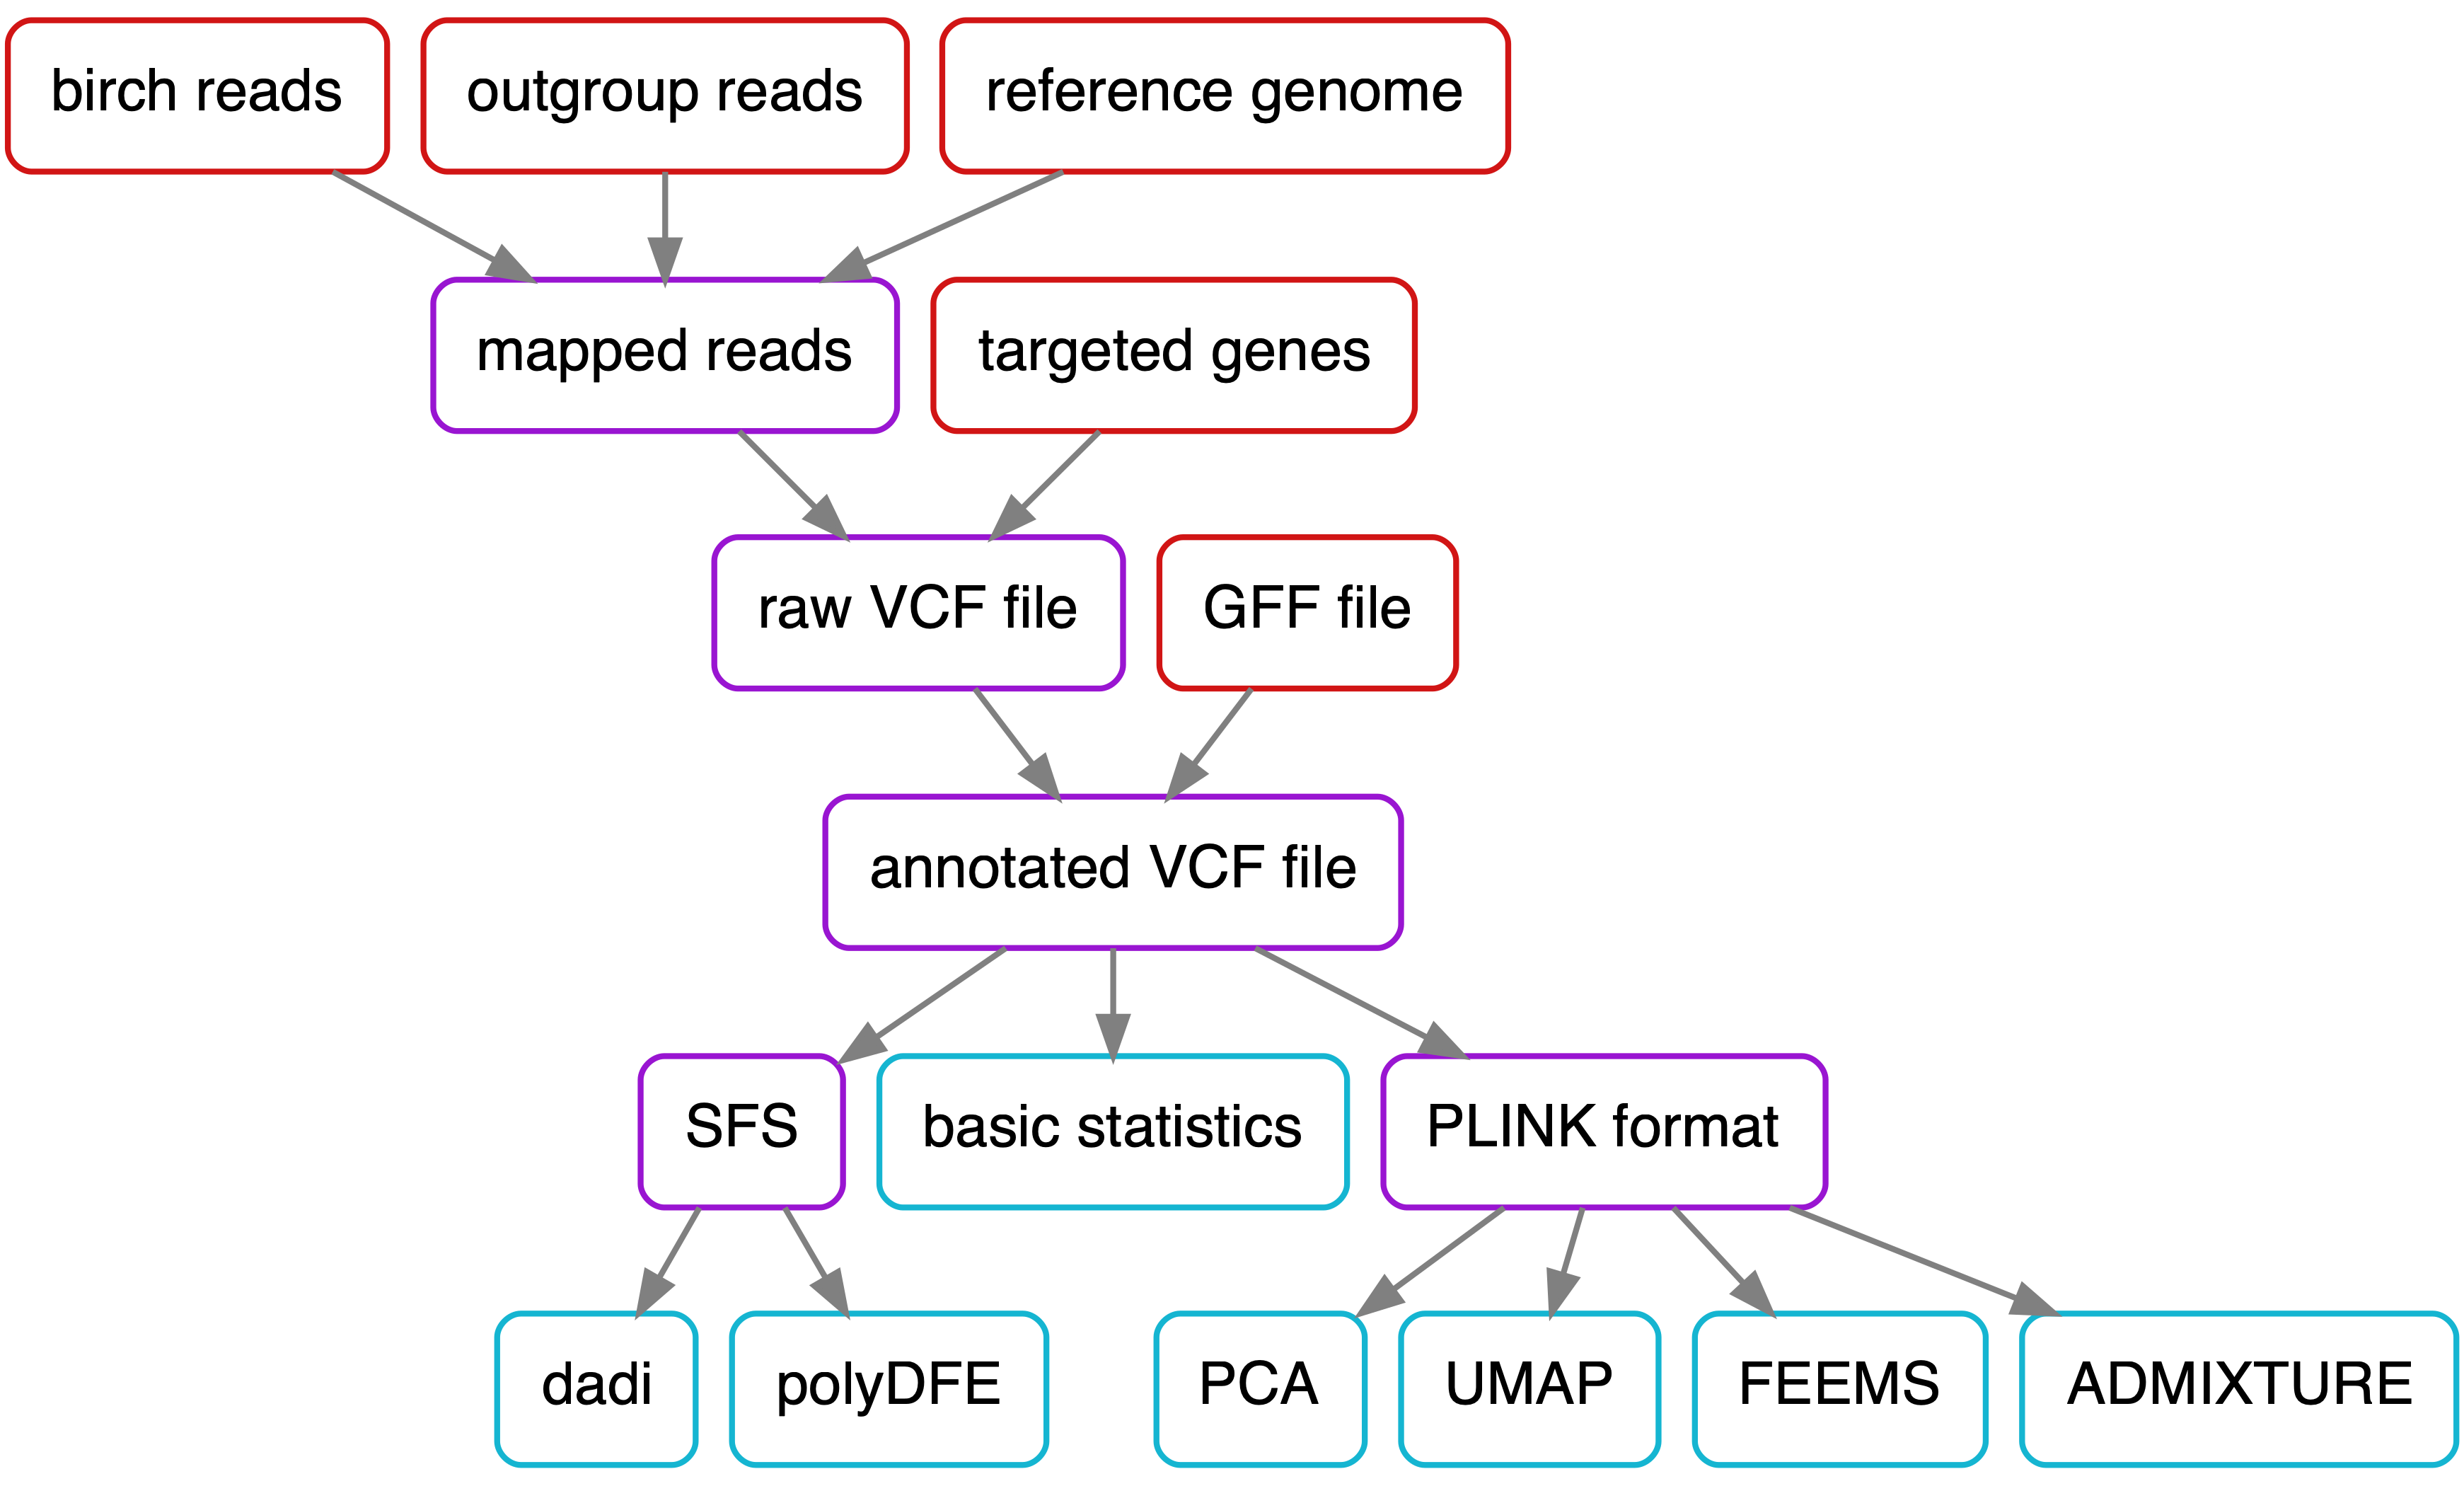
\includegraphics[width=\textwidth]{default/graphs/png/rulegraphs/schematics/pipeline.png}
        \caption{A schematic of the workflow. Resource data are marked red, intermediate steps are purple and final results are blue.}
        \label{fig:workflow_schematic}
    \end{figure}

    A schematic of the pipeline's workflow is shown in fig.~\ref{fig:workflow_schematic}. All analyses are based on bi-allelic \acrshort{snp} data whose derivation is as follows: The initial short reads were trimmed with Trimmomatic, mainly to remove the adapter sequences whence their quality was confirmed with FastQC \cite{trimmomatic,fastqc}. The mapping was done with \acrshort{bwa} using the \pendula{} reference genome \cite{ref-genome}. In doing so, we also expect to capture most variation within \pubescens{} whose polyploid origin likely involved \pendula{} (cf. section \ref{sec:species}). We then jointly called the variants using \acrshort{gatk}'s GVCF workflow to obtain a raw \acrshort{vcf} file (including monomorphic sites) \cite{gatk}. The variant calling was done twice: once treating all samples as diploid and once specifying their proper ploidy (\pubescens{} is tetraploid). This was done as some analyses cannot handle polyploid individuals. The resulting variants were subsequently hard-filtered according to \acrshort{gatk}'s best practices. The sites were then annotated with regards to their degeneracy and synonymy using custom scripts and the ancestral alleles were inferred with EST-SFS \cite{est-sfs}. All time-consuming tasks were parallelised to make the pipeline more efficient and scalable. The resulting annotated \acrshort{vcf} file was then used for the derivation of various sample sets that we used for further analyses. For each sample set configuration a separate \acrshort{vcf} file was created in order to easily run analyses over different sample sets. Sites with more than 50\% of missing values were removed from the sample sets if not specified otherwise. We then began by calculating some basic summary statistics like nucleotide diversity $\pi$, fixation index $F_{ST}$ and Tajima's $D$. The population structure was visualised with \acrshort{pca} and \acrshort{umap} (a non-linear dimension reduction technique) \cite{umap}. Migration surfaces were estimated with \acrshort{feems} \cite{feems}. Thereafter, we modelled the demographic history where \dadi{} was used to perform \acrfull{mle} on various demographic models which we were required to specify explicitly \cite{dadi}. Subsequently, polyDFE, which is also \acrshort{sfs}-based, was used to estimate the \acrfull{dfe} for different subpopulations which we then compared to each other \cite{polydfe}. For both analyses, we needed to differentiate between synonymous and non-synonymous sites to obtain a \acrfull{sfs} for each class. To additionally infer the \acrshort{dfe} for beneficial mutations and to increase the accuracy of the demographic modelling, we also needed to derive an unfolded \acrshort{sfs} by distinguishing between ancestral and derived alleles.

    \subsection{Nucleotide Diversity}
    \label{sec:pi}

    Table~\ref{tbl:pi} shows the nucleotide diversity $\pi$ and number of segregating sites $S$ for both birch species. Both values are significantly higher for \pubescens{} which is expected for polyploids, having more homologous sites where alleles can differ. This would be especially so for heteropolyploids with considerably diverged ancestors. The calculations were performed with \dadi{} and are \acrshort{sfs}-based implying that each sample could be treated with respect to its proper ploidy \cite{dadi}. We have $\pi = \frac{n}{n-1} \frac{1}{l}\Sigma_i 2p_i(1-p_i)$ where $n$ is the number of haplotypes, $l$ the total number of surveyed sites and $p_i$ the frequency of any of the two alleles at the $i$th segregating site \cite{gillespie}. This formula can be interpreted as the probability that two randomly chosen sites are segregating and can thus directly be applied to polyploid samples, the only difference being the increased number of haplotypes $n$ \cite{rick-durrett}. The ratio $\pi_N/\pi_S$ roughly denotes the fraction of non-synonymous mutations that were not removed by purifying selection i.e. the fraction of mutations that are selectively neutral or more strongly advantageous. Selectively neutral means here that selection is sufficiently weak for drift to predominate. We note that $\pi_N/\pi_S$ is slightly larger for \pubescens{} which could be explained by relaxed purifying selection in polyploids due to higher gene redundancy. It is also noteworthy that, for both species, $\pi_N/\pi_S$  is rather low in comparison to other tree species \cite{pi-plants,pi-spruce}.

    \begin{table}[H]
        \begin{center}
            \begin{tabular}{| l | l | l| }
                & \pendula{} & \pubescens{} \\
                $S$           & 39101      & 225531       \\
                $\pi$         & 0.00148    & 0.00600      \\
                $\pi_N$       & 0.00095    & 0.00290      \\
                $\pi_S$       & 0.00378    & 0.00974      \\
                $\pi_N/\pi_S$ & 0.251      & 0.298        \\
            \end{tabular}
        \end{center}
        \caption{The number of segregating sites $S$ and the nucleotide diversity $\pi$ over all sites. The synonymous and non-synonymous nucleotide diversity $\pi_S$ and $\pi_N$ were calculated over 4-fold and 0-fold degenerate sites, respectively.}
        \label{tbl:pi}
    \end{table}

    \subsection{Heterozygosity}
    \label{sec:het}

    The heterozygosity at a given locus describes the fraction of individuals that are heterozygous there. An expected heterozygosity $H$ can be calculated from a site's allele frequency assuming it is in \acrfull{hwe}. We have $H_i = 2p_i(1-p_i)$ where $p_i$ is the frequency of any allele at the $i$th bi-allelic site \cite{gillespie}. This is exactly the same formula as for the nucleotide diversity. However, in contrast, when calculating the actual observed heterozygosity we confine our comparison to the two loci within each diploid individual to see how they associate. A frequency distribution of the expected and observed heterozygosities for the two species can be found in the appendix (cf. fig.~\ref{fig:het}). By far most sites have values of $0$ as they are monomorphic. Under \acrshort{hwe}, at most half of all individuals are expected to be heterozygous provided that the sample size is greater than 1. $H_i$ thus ranges from $0$ to $0.5$ where $0.5$ is the theoretical maximum attained for $p = 0.5$. The observed heterozygosity exceeds $0.5$ in some cases which is expected due to sampling variance but can, in principle, be indicative of outbreeding or heterozygote advantage if it does so consistently. An excess of homozygotes is more common, however, and can be caused by dynamics like inbreeding or population structure \cite{gillespie}. For \pendula{}, the average observed heterozygosity is, in fact, slightly lower than its expectation (cf. fig.~\ref{fig:het_pendula}). This can partly be caused by non-random mating due to isolation by distance which is expected for stationary species of large geographical extend. In any case, the two distributions are in rather good agreement (note the logarithmic scale). \pubescens{}'s average observed heterozygosity, however, significantly exceeds its expectation which is, at least in part, due the bias introduced by calling it as a diploid (cf. fig.~\ref{fig:het_pubescens}). More precisely, it is caused by neglecting that polyploids are more likely to be heterozygous than diploids and by the overestimation of the frequency of rare alleles (cf. section \ref{sec:sfs} for a more detailed explanation). Site-wise p-values for the observed heterozygosity under \acrlong{hwe} can be found in fig.~\ref{fig:p_hwe}. Both the heterozygosity and p-values were calculated using PLINK \cite{plink, hwe-plink}.

    \clearpage


    \section{Derivation of Site-Frequency Spectra}
    \label{sec:sfs-derivation}
    
    \begin{figure}[ht]
        \centering
        \begin{subfigure}[b]{0.49\textwidth}
            \centering
            \includegraphics[width=\textwidth]{tetraploid/graphs/png/sfs/pendula/0fold_4fold/sfs.1D.20.unfolded.linear_tight_layout.png}
            \caption{\pendula{}}
            \label{fig:sfs_1d_pendula}
        \end{subfigure}
        \hfill
        \begin{subfigure}[b]{0.49\textwidth}
            \centering
            \includegraphics[width=\textwidth]{tetraploid/graphs/png/sfs/pubescens/0fold_4fold/sfs.1D.20.unfolded.linear_tight_layout.png}
            \caption{\pubescens{}}
            \label{fig:sfs_1d_pubescens}
        \end{subfigure}
        \par\bigskip
        \centering
        \begin{subfigure}[b]{0.32\textwidth}
            \centering
            \includegraphics[width=\textwidth]{tetraploid/graphs/png/sfs/pendula_pubescens/biallelic/sfs.2D.20.png}
            \caption{both species}
            \label{fig:sfs_2d_pendula_pubescens}
        \end{subfigure}
        \hfill
        \begin{subfigure}[b]{0.32\textwidth}
            \centering
            \includegraphics[width=\textwidth]{tetraploid/graphs/png/sfs/pendula/biallelic/sfs.2D.20.png}
            \caption{\pendula{}}
            \label{fig:sfs_2d_pendula}
        \end{subfigure}
        \hfill
        \begin{subfigure}[b]{0.32\textwidth}
            \centering
            \includegraphics[width=\textwidth]{tetraploid/graphs/png/sfs/pubescens/biallelic/sfs.2D.20.png}
            \caption{\pubescens{}}
            \label{fig:sfs_2d_pubescens}
        \end{subfigure}
        \caption{One- and two-dimensional unfolded site-frequency spectra down-projected to a sample size of 20. For the 1D case, we distinguish between 0- and 4-fold degenerate sites. We see that \pendula{} has many more high-frequency derived alleles than \pubescens{}. The ascertainment of the subpopulations shown on the axes of the 2D spectra is presented in the following section.}
        \label{fig:sfs}
    \end{figure}

    The \acrfull{sfs} is a powerful summary statistic of bi-allelic \acrshort{snp} variation. It provides information on the number of sites in each frequency class, i.e. $\xi = (\xi_i)^n_{i=0}$ where $\xi_i$ denotes the number of \acrshort{snp}s for which $i$ out of $n$ alleles are derived, i.e. not ancestral (cf. fig.~\ref{fig:sfs}). This is the definition of a so-called unfolded \acrshort{sfs} as it distinguishes sites with $i$ ancestral alleles from sites with $i$ derived alleles (cf. folded \acrshort{sfs} where frequency classes with $i$ and $n-i$ derived variants are collapsed). Unfolded spectra are much more informative. For example, they provide information on the number of high-frequency derived alleles which--when numerous--can be indicative of positive selection or population expansion. Both \dadi{} and polyDFE obtain their information by means of an \acrshort{sfs} and many summary statistics like $S$, $\pi$, $F_{ST}$ and Tajima's $D$ can be directly computed from it.

    In order to obtain an unfolded \acrshort{sfs}, we first need to infer the ancestral alleles which we did with the help of EST-SFS \cite{est-sfs}. For the inference, 50 ingroup and two outgroup samples were used which resulted in an \acrshort{sfs} that was sufficiently smooth. The ingroup subsampling was done without replacement whenever possible and both birch species were used as we deemed them sufficiently close in comparison to the outgroup species. The Kimura 2-parameter nucleotide substitution model was used according to the article's recommendation. There were initial problems determining the ancestral variants. EST-SFS calculates separate prior probabilities for each frequency class based on the maximum likelihood of the tree topologies for the two different ancestral states. This is being done to correct for the fact that high-frequency derived alleles are much less common than high-frequency ancestral ones (e.g. due to having more slightly deleterious mutations at low frequencies that have not yet been removed by purifying selection). The large variance of the number of samples among the frequency classes caused the prior to favour high-frequency derived alleles in some cases. This was especially true for small chunks of \acrshort{vcf} files that were initially used for the purpose of parallelisation. Choosing a larger number of ingroup samples also caused the variance to increase as we then have even more frequency classes containing fewer samples, each class receiving its own prior. On the other hand, reducing the ingroup sample size too much would introduce a lot of sampling variance. A moderate number of samples (i.e. 50) in addition to using all available \acrshort{snp}s at once, provided an \acrshort{sfs} that was sufficiently smooth (cf. fig.~\ref{fig:est_sfs}).

    \subsection{Degeneracy \& Synonymy}
    \label{sec:degeneracy-synonymy}

    \begin{figure}[ht]
        \centering
        \begin{subfigure}[b]{0.46\textwidth}
            \centering
            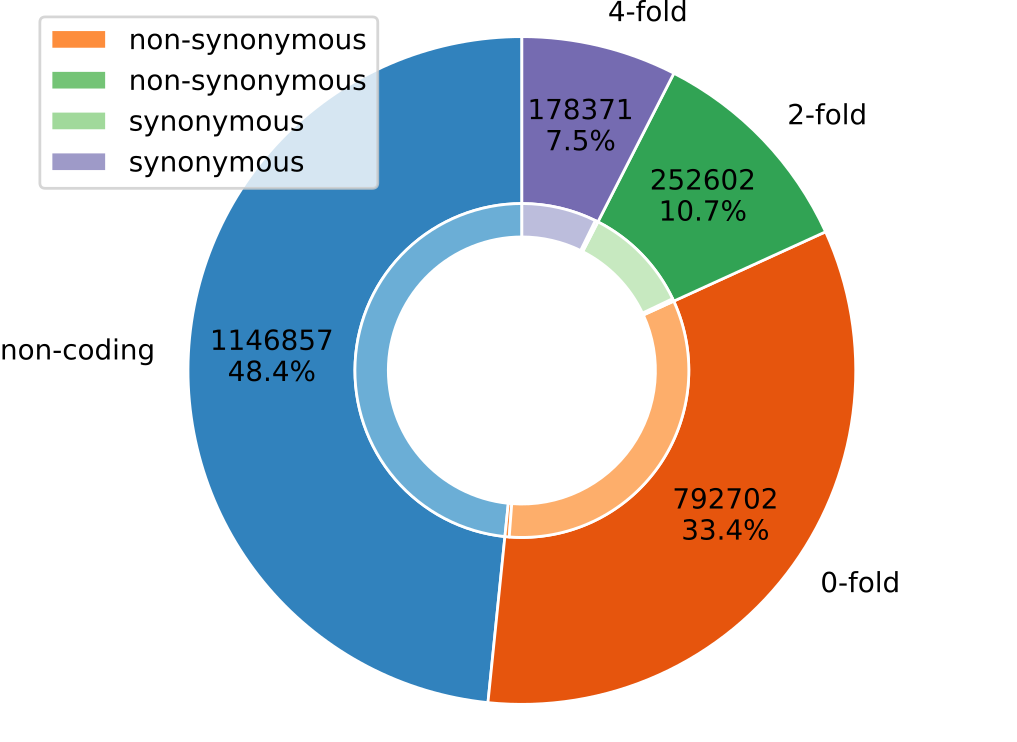
\includegraphics[width=\textwidth]{tetraploid/graphs/png/degeneracy/birch/degeneracy.png}
            \caption{Degeneracy}
            \label{fig:degeneracy}
        \end{subfigure}
        \hfill
        \begin{subfigure}[b]{0.52\textwidth}
            \centering
            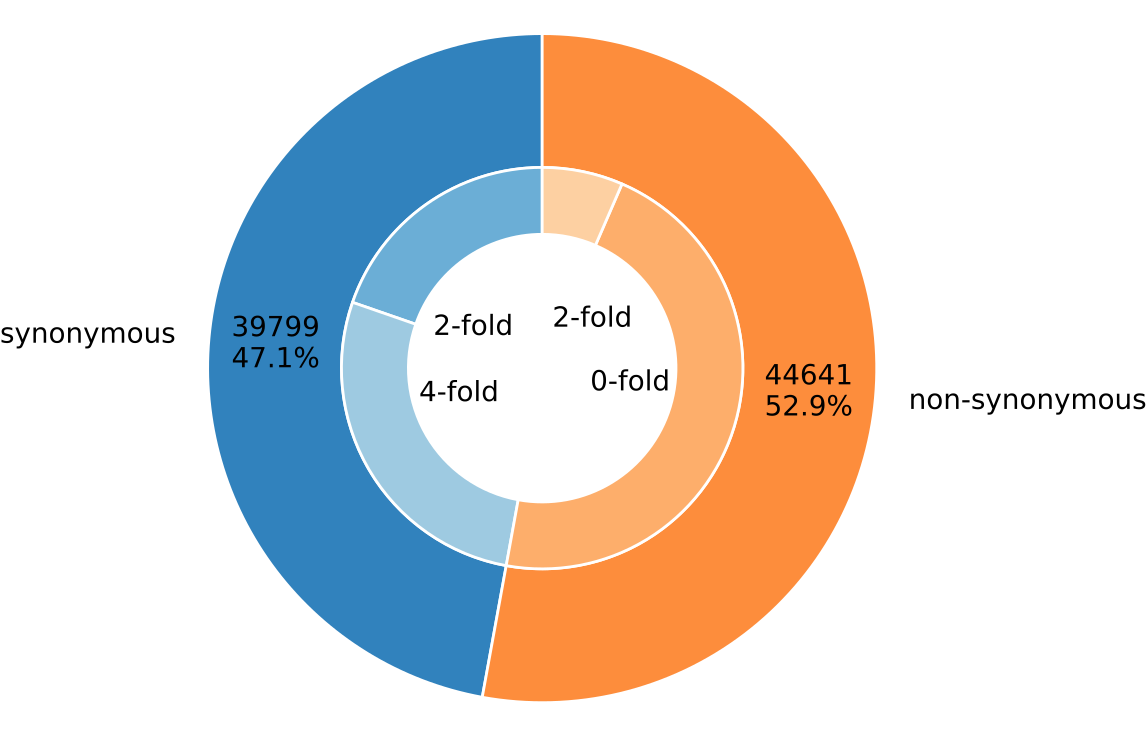
\includegraphics[width=\textwidth]{tetraploid/graphs/png/synonymy/birch/synonymy.png}
            \caption{Synonymy}
            \label{fig:synonymy}
        \end{subfigure}
        \caption{Classification of all targeted sites (left) as well as all coding bi-allelic sites (right). The whitish stretches in the inner disk of the left figure indicate the number of monomorphic sites.}
        \label{fig:synonymy_degeneracy}
    \end{figure}

    We may want to restrict our analyses to sites for which we have a more narrow notion of the underlying forces acting on them. For example, we might only be interested in sites not subject to direct selection or to compare different classes of sites. Coding sites can be classified in several ways: A polymorphic site is said to be synonymous if all alleles code for the same amino acid--it is said to be non-synonymous otherwise. Synonymous sites are often assumed to not be affected by direct selection so that their variational patterns are purely shaped by demography, drift and their genomic background. This is useful when demography is everything we are interested in or when investigating how selection affects variation by controlling for demography. For sites not necessarily polymorphic, we can instead look at their degeneracy, i.e. the potential of a point mutation to change the amino acid coded for. We distinguish between 0-fold, 2-fold, 4-fold degenerate sites. 4-fold degeneracy means that no mutation would result in a different amino acid, i.e. all mutations are silent. At 0-fold sites, any mutation would produce an amino acid change while at 2-fold sites, only two out of three possible mutations would cause such a change.

    Fig.~\ref{fig:synonymy_degeneracy} shows how degeneracy and synonymy are allocated to all targeted sites and all coding bi-allelic sites, respectively. 0-fold degenerate sites seem to be much more common than 2-fold and 4-fold degenerate sites which can readily be confirmed by looking at a coding table. We nonetheless have a substantial amount of synonymous sites which can be explained by noting that they fix more easily (most non-synonymous mutations being deleterious). In the same vein, one might expect there to be more 2-fold non-synonymous than synonymous sites as the majority of changes (two out of three) are non-synonymous, after all. Again, we have to note that non-synonymous mutations are much more likely to get removed by purifying selection. The results obtained are based on custom scripts as no appropriate tool for determining the sites' degeneracy could be found. The synonymy of the mutations as well as the resulting codons were compared with results from VEP to confirm their validity \cite{vep}.

    \subsection{Site Frequency Spectrum}
    \label{sec:sfs}

    Unfolded site-frequency spectra for 0-fold and 4-fold degenerate sites down-projected to a sample size of 20 are shown in fig.~\ref{fig:sfs}. Interestingly, \pendula{} has many more high-frequency derived alleles for both classes. This u-shape can, in theory, be explained by population expansion, population structure, multiple-merger coalescents or gene flow from disparate populations \cite{u-shape-gene-flow}. In the case of gene flow, we would rather expect \pubescens{} to have a u-shaped spectrum as we expect it to have a higher introgression rate. Population structure is unlikely to be the culprit either as not a lot of it can be found in birch. Another explanation could be ancestral misidentification but both species are based on the same ancestral states and \pubescens{} rather exhibits a deficit of high-frequency derived alleles. \pubescens{} furthermore has a relatively large amount of low-frequency derived alleles potentially owing to reduced purifying selection brought about by higher gene redundancy.

    Treating \pubescens{} as diploid when calling the variants biased the SFS toward having more intermediate- and fewer low-frequency alleles (cf. fig.~\ref{fig:sfs_ploidy_calling_differences}). This is easiest explained by observing that low-frequency alleles will likely only have one copy in heterozygous individuals (assuming no strong deviation from \acrshort{hwe}). Treating these individuals as diploid assumes that half of their haplotypes contain that allele, thus overestimating its frequency. Equivalently, we can say that for low-frequency alleles, the number of occurrences (i.e. roughly one per heterozygote) is counted to be the same but the total number of haplotypes is lower when assuming diploidy instead of a higher ploidy.

    2-dimensional (2D) frequency spectra provide plenty of information on the relatedness of two populations as they encode how their allele frequencies are associated site-wise. In general, the more recent their common ancestry or the more migration, the more sites we find in classes with similar frequencies. In fig.~\ref{fig:sfs}, we can also see down-projected 2D frequency spectra for different sample sets. The spectrum in fig.~\ref{fig:sfs_2d_pendula_pubescens} is rather spread-out, i.e. very disparate frequencies can be observed per site, which is indicative of little migration or relatedness. This makes perfect sense as we are looking at two separate species here and is in strong contrast to the spectra for \pendula{} and \pubescens{} whose subpopulations are highly admixed (cf. fig.~\ref{fig:sfs_2d_pendula} \& \ref{fig:sfs_2d_pubescens}). These spectra also show much more symmetry about the line $x=y$, indicating similar allele frequencies in both populations.

    \clearpage

    \section{Population Structure}
    \label{sec:population-structure}

    Population structure can be shaped by many forces, be it through local adaption, mating structure or demographic history. In this section we examine the structure and migration between and within populations of our two species. We do this by means of dimensionality reduction (\acrshort{pca} \& \acrshort{umap}), summary statistics ($F_{ST}$) and model-based approaches (\mbox{ADMIXTURE}, \acrshort{feems}). We mainly expect to find traces left behind by the postglacial recolonisation of different populations and adaption to different climatic environments as observed for Norway spruce \cite{spruce-demography}.

    \subsection{PCA \& UMAP}
    \label{sec:pca-umap}

    \begin{figure}[!htbp]
        \centering
        \begin{subfigure}[b]{0.48\textwidth}
            \centering
            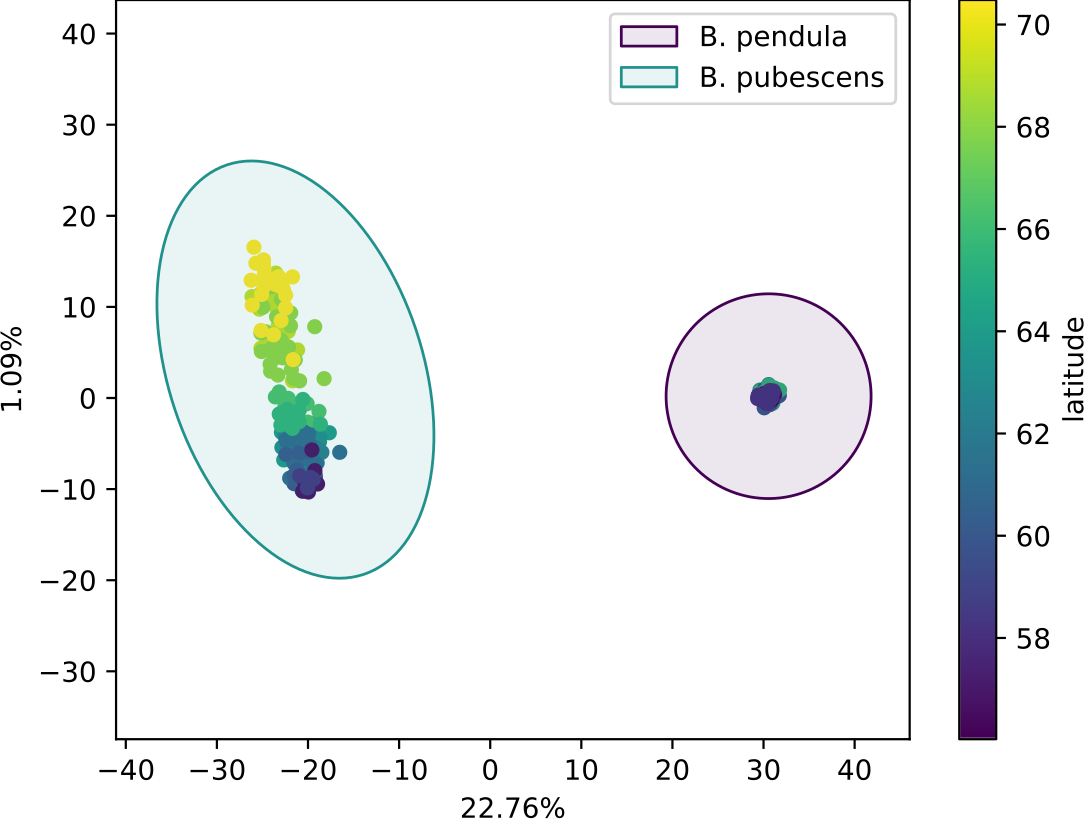
\includegraphics[width=\textwidth]{default/graphs/png/pca/birch/biallelic/pca_marked.png}
            \caption{\acrshort{pca}}
            \label{fig:pca_pendula_pubescens}
        \end{subfigure}
        \hfill
        \begin{subfigure}[b]{0.49\textwidth}
            \centering
            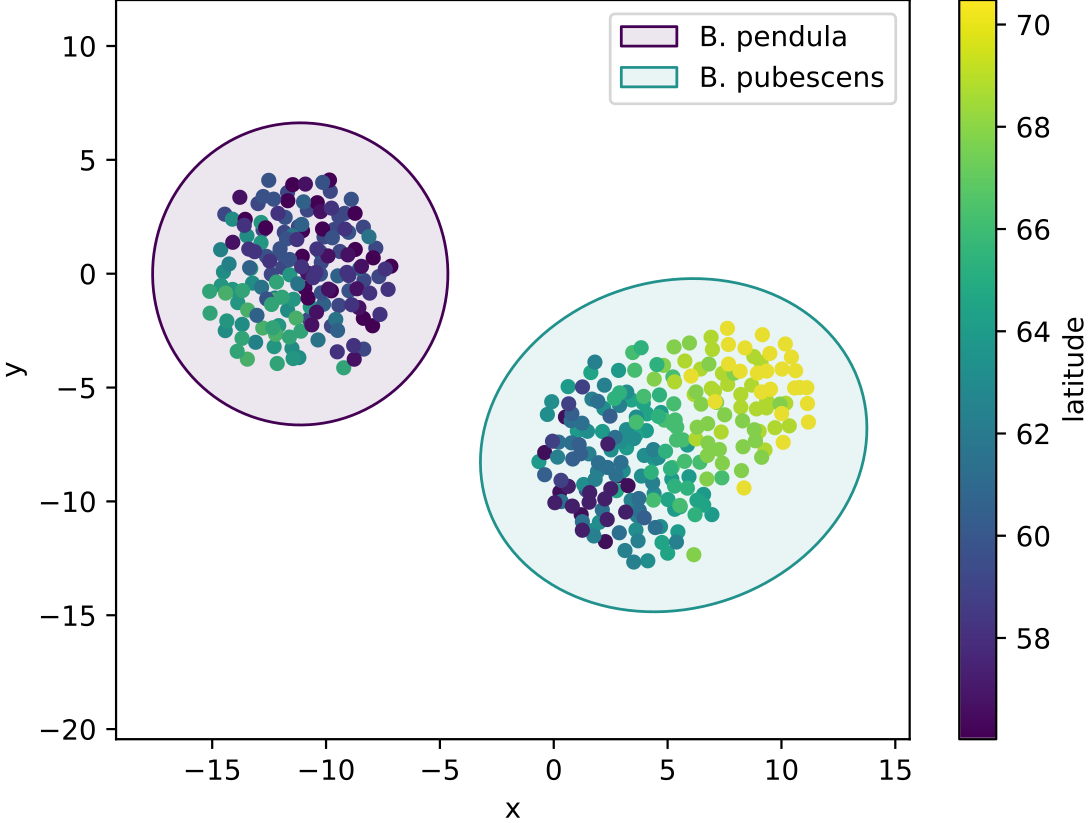
\includegraphics[width=\textwidth]{default/graphs/png/umap/birch/biallelic/umap_marked.png}
            \caption{\acrshort{umap}}
            \label{fig:umap_pendula_pubescens}
        \end{subfigure}
        \par\bigskip
        \centering
        \begin{subfigure}[b]{0.492\textwidth}
            \centering
            \includegraphics[width=\textwidth]{default/graphs/png/pca/pendula/synonymous/pca_tight_layout.png}
            \caption{\pendula{}}
            \label{fig:pca_synonymous_pendula}
        \end{subfigure}
        \hfill
        \begin{subfigure}[b]{0.49\textwidth}
            \centering
            \includegraphics[width=\textwidth]{default/graphs/png/pca/pubescens/synonymous/pca_tight_layout.png}
            \caption{\pubescens{}}
            \label{fig:pca_synonymous_pubescens}
        \end{subfigure}
        \caption{\acrshort{pca} (\subref{fig:pca_pendula_pubescens}) and \acrshort{umap} (\subref{fig:umap_pendula_pubescens}) plots on the set of bi-allelic sites. There is a clear separation between the two species. For \acrshort{umap}, the \texttt{spread} and \texttt{min\_dist} parameters were set to 2 and 1.5, respectively. There are also \acrshort{pca} plots on the set of synonymous sites for \pendula{} (\subref{fig:pca_synonymous_pendula}) and \pubescens{} (\subref{fig:pca_synonymous_pubescens}), separately. Two clusters are apparent for each species, especially for \pubescens{}.}
        \label{fig:pca}
    \end{figure}

    \acrfull{pca} employs linear dimensionality reduction thus retaining the proportions among distances and providing information on how much of the total variance is accounted for by each dimension. The \acrfull{umap} analysis is more customisable at the cost of interpretability as the principal dimensions need not be linear. Figs.~\ref{fig:pca_pendula_pubescens} \& \ref{fig:umap_pendula_pubescens} show \acrshort{pca} and \acrshort{umap} plots for bi-allelic sites where both species are considered in tandem. There is a clear delineation separating the species indicating that hybrids are relatively rare (with the exception of one or two intermediate samples). Considering the \acrshort{pca} plot, we see that roughly 20\% of the total variance is explained by the type of species. The second principal component is much smaller with 1\% and seems to account for latitudinal differentiation in \pubescens{}. The \acrshort{umap} plot looks similar but allows for a more detailed picture within each species brought about by specifying a minimum distance between samples (cf. fig.~\ref{fig:umap_pendula_pubescens}). Here we can also observe weak latitudinal differentiation for \pendula{}.

    The two principal components of the intra-specific plots naturally account for much less of their total variance, being far more homogenous (cf. figs.~\ref{fig:pca_synonymous_pendula} \& \ref{fig:pca_synonymous_pubescens} where sites were restricted to be synonymous for better visibility). For each species we can roughly see two clusters. This is especially apparent for \pubescens{} where we observe a scarce region between the clusters and along the first principle component (cf. x-axis in fig.~\ref{fig:pca_synonymous_pubescens}). A smooth latitudinal gradient is also apparent along the same component indicating a northern and southern subpopulation. Restricting instead to bi-allelic or non-synonymous sites, the \acrshort{pca} and \acrshort{umap} plots look very similar for \pubescens{} (cf. figs.~\ref{fig:pca_pendula_pubescens_separate} - \ref{fig:umap_biallelic_pendula_pubescens_separate}). For \pendula{}, the second principal component varies latitudinally but much less smoothly so (cf. y-axis in fig.~\ref{fig:pca_synonymous_pendula}). Using the set of non-synonymous sites instead, we do not observe any latitudinal gradient along the two principal components (cf. fig.~\ref{fig:pca_nonsynonymous_pendula}). This could indicate that the observed population structure in \pendula{} is more due to past demography and not a result of local adaption . This could be in agreement with the postglacial recolonisation of several distinct populations.

    A subpopulation division seems appropriate, whose boundary was drawn along the 64th and 65th parallel for \pendula{} and \pubescens{}, respectively (cf. fig.~\ref{fig:locations}). Interestingly, this boundary roughly corresponds to a transition from humid continental climate in the south to subarctic climate in the north according to the Köppen classification system. A boundary at a similar latitude was also determined for Norway spruce (cf. section \ref{sec:expectations}) \cite{spruce-demography}. We also note that there is overall little population structure. Care has to be taken not to over-interpret the latitudinal gradient as the data itself mainly varies along that direction. Without prior knowledge or the scarce region separating the two clusters for \pubescens{}, we could merely be led to conclude that there is isolation by distance.

    \subsection{ADMIXTURE}
    \label{admixture}

    To corroborate and refine the population clustering deduced from the \acrshort{pca} and \acrshort{umap} plots, the model-based clustering tool \mbox{ADMIXTURE} was used \cite{admixture}. As output we obtain the percental allocation to the specified clusters per individual with the number of clusters being specified by parameter $K$. The set of bi-allelic sites was filtered for sites in strong \acrshort{ld} using PLINK where we used a window and step size of 500 and 50 \acrshort{snp}s, respectively as well as an $r^2$ threshold of 0.2. To detect the rather weak population structure of \pendula{}, $r^2=0.99$ was used instead, for sufficiently many sites to remain.
    
    The results indicate a subpopulation structure very similar to that in the previous section (cf. fig.~\ref{fig:pca_admixture}). However, \mbox{ADMIXTURE}'s cross validation procedure favours only a single cluster for the intra-specific cases (cf. fig.~\ref{fig:admixture_cv_error_pendula_pubescens}). Looking at the bar plot in fig.~\ref{fig:admixture_barplot_pendula_pubescens_2}, it is apparent that there is admixture from \pendula{} into (mainly southern) \pubescens{} populations but not vice versa. This is entirely consistent with our expectations on diploid-tetraploid gene flow \cite{stebbins,birch-unidirectional-introgression}. The southern and northern subpopulations within each of the two species are furthermore visibly admixed although there is considerably more admixture near the contact zone for \pubescens{} (cf. figs.~\ref{fig:admixture_barplot_pendula_2} \& \ref{fig:admixture_barplot_pubescens_2}). Admixture among \pendula{}'s subpopulations, on the other hand, is apparent much farther away from the contact zone, notably from the northern population far into the south (cf. fig.~\ref{fig:admixture_barplot_pendula_2}). This is likely due to \pendula{}'s very weak population structure. No sensible clustering was evident for larger values of $K$ (cf. figs.~\ref{fig:admixture_barplot_pendula_pubescens_4}, \ref{fig:admixture_barplot_pendula_3} \& \ref{fig:admixture_barplot_pubescens_3}).

    \begin{figure}[H]
        \centering
        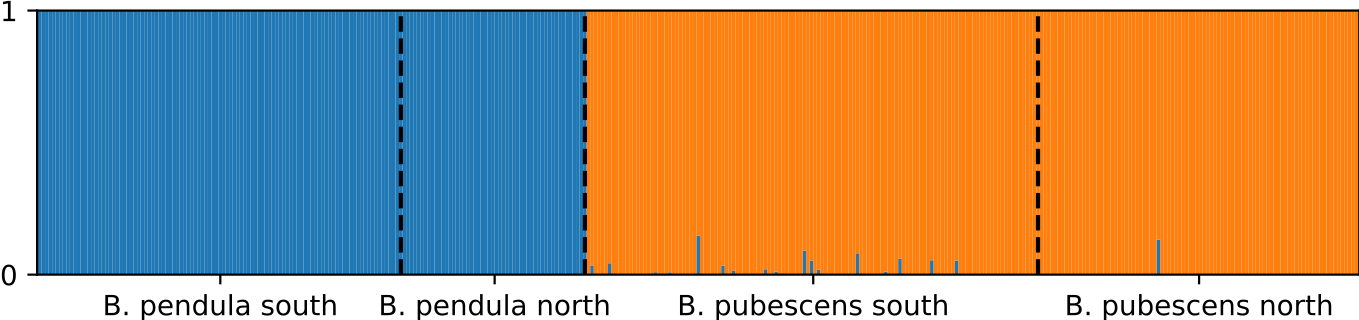
\includegraphics[width=\textwidth]{default/graphs/png/admixture/pendula_pubescens/biallelic/barplot.2.4.png}
        \caption{Bar plot for both species using $K=2$. The samples are first sorted by the displayed (\mbox{ADMIXTURE}) subpopulations and second by latitude in ascending order. The clustering adheres to the species boundary. We also observe admixture from \pendula{} into (mainly southern) \pubescens{} individuals but not vice versa.}
        \label{fig:admixture_barplot_pendula_pubescens_2}
    \end{figure}

    \subsection{$F_{ST}$}
    \label{sec:fst}

    \begin{table}[H]
        \begin{center}
            \begin{tabular}{| l | l | l |}
                & mean $F_{ST}$ & weighted $F_{ST}$ \\
                \pendula{} / \pubescens    & 0.0335        & 0.1951            \\
                \pendula{} north / south   & 0.0026        & 0.0119            \\
                \pubescens{} north / south & 0.0025        & 0.0111            \\
            \end{tabular}
        \end{center}
        \caption{Weighted as well as average $F_{ST}$ per site.}
        \label{tbl:fst}
    \end{table}

    Table~\ref{tbl:fst} shows the population differentiation given by the fixation index $F_{ST}$ which is a measure of subpopulation differentiation. The $F_{ST}$ can be defined for a single site by $\sigma^2_{p_i}/\sigma^2_p$ where $\sigma$ denotes the variance and $p$ and $p_i$ denote the frequency of a certain allele in the overall population and in the $i$th subpopulation, respectively. The denominator $\sigma^2_p = pq$ describes the variance of the site's allelic state in the overall population and the numerator $\sigma^2_{p_i} = \sum_j (p_j - p)^2 / n$ the variance across the $n$ different subpopulations (assuming they are of equal size)\cite{gillespie}. It is thus measuring how much of the total variance in allele frequencies is attributable to the variance across subpopulations. An $F_{ST}$ of $0$ indicates that there is no subpopulation differentiation of any kind while an $F_{ST}$ of $1$ would mean that all variance is due to subpopulation structure, i.e. there is no variance within subpopulations. \pubescens{} was treated as a diploid for the site-wise calculations as VCFtools cannot handle polyploidy \cite{vcftools}. The weighted $F_{ST}$ was inferred from the \acrshort{sfs} using \dadi{}, and thereby properly reflects the different ploidies \cite{dadi}. Both tools base their calculations on the method of Weir and Cockerham who advocate the weighted method \cite{weir-cockerham}. We observe rather little differentiation between the northern and southern subpopulations within each of the two species as expected. A more marked subpopulation differentiation for \pubescens{} as suggested by the \acrshort{pca} plots (cf. fig.~\ref{fig:pca}) is not reflected in the values. Frequency distributions of the site-wise $F_{ST}$ for \pendula{} and \pubescens{} can be found in the appendix (cf. fig.~\ref{fig:fst}).

    \subsection{FEEMS}
    \label{sec:feems}

    \begin{figure}[ht]
        \centering
        \begin{subfigure}[b]{0.47\textwidth}
            \centering
            \frame{\includegraphics[width=\textwidth,height=17em]{default/graphs/png/feems/pendula/no_very_low_freqs/migration_surfaces_lambda_10_buffer_1.png}}
            \caption{\pendula{}}
            \label{fig:feems_no_very_low_freqs_pendula_lambda_10}
        \end{subfigure}
        \hfill
        \begin{subfigure}[b]{0.47\textwidth}
            \centering
            \frame{\includegraphics[width=\textwidth,height=17em]{default/graphs/png/feems/pubescens/no_very_low_freqs/migration_surfaces_lambda_10_buffer_1.png}}
            \caption{\pubescens{}}
            \label{fig:feems_no_very_low_freqs_pubescens_lambda_10}
        \end{subfigure}
        \caption{Migration surface plots for both species with smoothing parameter $\lambda = 10$. The red and blue colours indicates below-average and above-average migration, respectively. Note that a buffer region has been added here for reasons of visibility. Unbuffered plots can be found in the appendix (cf. fig.~\ref{fig:feems_no_buffer_no_low_freqs}).}
        \label{fig:feems_no_very_low_freqs_lambda_10}
    \end{figure}

    To determine the migration intensity between samples, \acrshort{feems} was used, which employs a model-based approach \cite{feems}. Performing the analysis, all samples are first assigned to the nearest node of the underlying spatial grid (cf. fig.~\ref{fig:feems_no_very_low_freqs_lambda_10}). The smoothing parameter $\lambda$ controls how much emphasis is put on local structure and can be determined with leave-one-outcross-validation (cf. fig.~\ref{fig:feems_cv_error_no_very_low_freqs}). That is, one node is held out from the set of nodes for which the genotype is inferred from the remaining nodes under consideration of the estimated migration intensity between them. The final cross-validation error is then taken to be the average difference between expected and inferred genotype for each held-out node. Using warm starts for the cross-validation, where runs are initialised with the migration rates of the previous run, did not produce very different values of $\lambda$ compared to cold starts where each run uses the same initialisation. Increasing the extend of the underlying grid by using a buffer of size 1 was furthermore necessary for the results to be better visible. Removing the buffer region, the results are optically less visible but we keep observing above and below-average migration in the south and north, respectively (cf. fig.~\ref{fig:feems_no_buffer_no_low_freqs}). Preparing the data, sites with an allele frequency lower than 1\% and a missingness greater than 50\% were removed. The analysis was repeated several times for different thresholds yielding similar results although the cross-validation procedure often produced implausible values of $\lambda$ (cf. fig.~\ref{fig:feems_no_very_low_freqs_lambda_cv}}). We thus had to look for features in the migration surfaces that are visible for a large set of smoothing values and resort to common sense to gauge when a plot was overfitted. This approach is also recommended in the underlying article \cite{feems}. Choosing  $\lambda=10$ for both species provided rather smooth migration surfaces whose rates did not change unreasonably abrupt (cf. fig.~\ref{fig:feems_no_very_low_freqs_lambda_10}). Choosing smaller values, we start to observe small isolated low-migration patches around some of the nodes and very abrupt changes in migration intensity, which is indicative of overfitting (cf. fig.~\ref{fig:feems_no_very_low_freqs_lambda_0.1}).

    Additional care has to be taken when interpreting these results as all the samples are distributed along a single latitudinal gradient which can potentially lead to artifacts. In fig.~\ref{fig:feems_no_very_low_freqs_pubescens_lambda_10} and more clearly in fig.~\ref{fig:feems_no_very_low_freqs_pubescens_lambda_0.1}, we observe a lower migration intensity along the axis comprising the samples compared to the buffer region for which there exist no additional samples. This does not seem entirely sensible and could be resolved by obtaining more samples that vary longitudinally. We can also argue, however, that migration between more distant populations is taken into account in the outer buffer regions where a lower migration rate would make sense.

    In summary, we observe above-average migration in the south and below-average migration in the north. A partial barrier to gene flow, separating the northern and southern subpopulations apparent in the \acrshort{pca} plots, is not visible. Migration seems to be rather uniform, especially for \pendula{} which can be interpreted to be in line with the less marked population structure in fig.~\ref{fig:pca_synonymous_pendula}. The relatively homogenous migration rates also agree with there being overall little population structure. By choosing sufficiently large smoothing values, however, all data can be made to look homogenous. Nevertheless, it is reassuring that we obtain a similar picture for both species and different allele frequency cut-offs.

    \clearpage


    \section{Demographic History}
    \label{sec:demographic-history}

    Ignoring selection and drift, what we are left with is a species' demography. Demography can be influenced by many factors like geographical boundaries, heterogeneous environmental pressures or mating system. In our case, we are mainly interested in population size changes and gene flow between different populations. We assume the mating structure to play only a minor role--birches being quite promiscuous with regards to where their pollen land. Here we attempt to find population size expansion after the \acrlong{lgm} and possibly gene flow between \pendula{} and \pubescens{} (cf. sections \ref{sec:species} \& \ref{sec:expectations}).

    For our demographic analysis, we used an \acrshort{sfs}-based tool called \dadi{} which explicitly models demographic scenarios using diffusion approximations \cite{dadi}. The underlying equation essentially is a deterministic partial differential equation modelling the effects of drift, population size, selection and migration on the allele frequencies. Independent Poisson likelihoods are used for the number of sites in each frequency class. For our results not to be confounded by selection, we confine our analysis to synonymous sites which we assume to be neutrally-evolving. There being so many possible demographic scenarios, a particularly shaped SFS can result in many different ways. Choosing a particular model, e.g. a set of discrete population size changes in one population, we force the \acrshort{sfs} to be modelled in only that manner.

    \subsection{Methods}

    We consider both one and two-population scenarios, with variable and fixed time and discrete as well as continuous population size changes (cf. fig.~\ref{fig:schematic_scenarios_dadi} for a schematic of the sample sets and population scenarios that were used). In the one-population scenarios we mostly consider population size changes whereas we can include migration in the two-population scenarios. For the fixed-time scenarios, the time has been fixed to roughly coincide with the end of the \acrlong{lgm} (about 16\,000 BP). Variable-time models should provide better fits in most cases but fixing the time was nonetheless considered useful as it facilitated model comparison. That being said, the time since the \acrshort{lgm} has to be interpreted with caution as our parameters are scaled by mutation rate and effective population size for which no accurate estimates are available.

    A mutation rate of $\mu = 10^{-9}$ per site per generation and generation time of $t=20$ years was used \cite{jarkko}. The effective population size $N_e$ was determined to be $945\,883$, $2\,433\,981$ and $2\,235\,669$ for \pendula{} and \pubescens{} and both species together, respectively. Here we calculated $N_e$ based on the synonymous nucleotide diversity (i.e. $\pi_N = 4 N_e \mu \Leftrightarrow N_e = \pi_N/(4\mu)$). This is a rather rough estimate and was solely used for the fixed-time scenarios. \pubescens{}' effective population size is likely higher than \pendula{}'s owing to a larger number of haplotypes per individual and introgression from \pendula{} and \nana{}. However, the above formula for $\pi$ can be interpreted as $\mu$ multiplied by twice the expected coalescent time for two homologous sites. These coalescent times are likely higher between \pubescens{}' two sub-genomes which can lead to inflated estimates of $N_e$ when assuming otherwise.

    \begin{table}[H]
        \begin{center}
            \begin{tabular}{| l | l | l | l | l | l |}
                parameter       & symbol & lower bound & upper bound & scaling \\
                population size & $\nu$  & 0.001       & 1000        & $N_e$   \\
                migration rate  & $m$    & 0           & 2           & $2N_e$  \\
                time            & $t$    & 0           & 1           & $2N_e$  \\
            \end{tabular}
        \end{center}
        \caption{Parameter bounds. Parameter $\nu$ is a fraction relative to the initial population size $N_e$. Migration is given by $m=2N_e m_f$ where $m_f$ is the fraction of individuals in the recipient population that come from the other population each generation. It is thus the effective number of individuals that migrate. Time is given by $t$ in units of $2N_e$ generations.}
        \label{tbl:param_bounds}
    \end{table}

    Table~\ref{tbl:param_bounds} shows all commonly used parameters as well as a description and their upper and lower bounds. Most of the models are nested allowing for model comparison by means of \acrlong{lrt}s (LRTs). Apart from the likelihood, we also use the average Anscombe residual as an estimator of the models' goodness of fit. This quantity is not directly optimised for but should provide a good indication. The Anscombe residual quantifies the difference between the number of modelled and observed sites per frequency class \cite{dadi-docs}. It also normalises this difference with respect to its variance in addition to making it follow a normal distribution.

    The parameter estimation for \dadi{} consists of two steps (cf. fig.~\ref{fig:dadi_workflow}). First, to obtain solid estimates, a semi-global optimisation routine was performed by using 1000 parallelised \acrshort{bfgs} local-optimisation runs that were randomly distributed in parameter space. For parameters with very wide bounds, a log-uniform sampling distribution was used. Basin hopping, a global optimisation technique, was also tested but did not yield satisfactory results. Bootstrap samples were generated using \dadi{}'s helper functions by sampling with replacement from several hundred contiguous chunks the genome was partitioned into. Using chunks instead of single sites is justified as it increases the samples' independence, linkage within chunks being greater than between \cite{dadi-docs}. A good chunk size was found to be 1\,000\,000 bases across, smaller sizes producing too many empty chunks. The bootstrap samples were then each initialised with the best result from the initial optimisation routine and optimised semi-locally using 5-10 separate \acrshort{bfgs} runs of sequentially perturbed initial values. The first run produced the highest likelihood in most cases. \dadi{}'s standard deviation estimates by means of the \acrlong{gim} deviated far from the manual bootstrap estimates.

    \subsection{One-Population Scenarios}

    \begin{table}[H]
        \begin{center}
            \resizebox{\textwidth}{!}{
                \setlength\tabcolsep{7pt}
                \begin{tabular}{|l|l|l|l|l|l|}
                    scenario          & $log(L)$                   & t                            & $\nu_0$                          & $\nu_1$                  &                                       \\
                    constant size     & -108\,$\pm$\,9.5           & 0.33\phantom{0}\,$\pm$\,0.04 & 2.4\phantom{000}\,$\pm$\,0.13       &              &                            \\
                    linear growth     & -88\phantom{0}\,$\pm$\,6.0 & 0.21\phantom{0}\,$\pm$\,0.02 & 0.0012\,$\pm$\,0.00059 &              & $c$\,=\,488\phantom{0.}\,$\pm$\, 111       \\
                    exp growth        & -92\phantom{0}\,$\pm$\,7.1 & 0.049\,$\pm$\,0.032          & 0.0034\,$\pm$\,0.0035            &              & $e$\,=\,25\phantom{0.0}\,$\pm$\,4.6       \\
                    1-size change     & -83\phantom{0}\,$\pm$\,5.4 & 0.067\,$\pm$\,0.029          & 0.0044\,$\pm$\,0.0017  & 39\phantom{0}\,$\pm$\,32  & $s$\,=\,0.22\phantom{0}\,$\pm$\,0.071   \\
                    constant size LGM & -115\,$\pm$\,10            & 0.17                         & 2.7\phantom{000}\,$\pm$\,0.21    &                          &                                       \\
                    linear growth LGM & -93\phantom{0}\,$\pm$\,7.5 & 0.17                         & 0.001\phantom{0}\,$\pm$\,2e-05    &              & $c$\,=\,346\phantom{0.}\,$\pm$\,15       \\
                    exp growth LGM    & -93\phantom{0}\,$\pm$\,7.2 & 0.17                         & 0.016\phantom{0}\,$\pm$\,0.00047 &              & $e$\,=\,18\phantom{0.0}\,$\pm$\,2.1       \\
                    1-size change LGM & -82\phantom{0}\,$\pm$\,5.0 & 0.17                         & 0.0013\,$\pm$\,0.00025           & 354\,$\pm$\,50 & $s$\,=\,0.015\,$\pm$\,0.0026 \\
                \end{tabular}}
        \end{center}
        \caption{1D population scenarios for \pendula{} after the \acrshort{lgm}. The population size grows from $\nu_0$ in the past to $\nu_1$ in the present during time $t$. Parameter $s$ denotes the fraction of $t$ at which a discrete time change occurs and $c$ and $e$ parametrise the slope in the continuous growth scenarios. These parametrisations reduce to the constant size scenario and are thus appropriate for \acrshort{lrt}s. The standard deviation has been calculated from 100 \acrfull{bca} bootstraps and the point estimates are the average values thereof.}
        \label{tbl:1d_dadi}
    \end{table}

    Table~\ref{tbl:1d_dadi} shows the maximum likelihood estimates of some one-population scenarios for \pendula{}. The standard deviation is reasonbly small indicating that a good local optimum could be found. The observed and modelled \acrshort{sfs} as well as the population size trajectory of the fixed-time scenarios in table~\ref{tbl:1d_dadi} are illustrated in figs.~\ref{fig:one_pop_size_change_since_ice_age_pendula} \& \ref{fig:constant_pop_size_since_ice_age_pendula} - \ref{fig:exp_pop_growth_since_ice_age_pendula}. The best fit was achieved by modelling a single population size change. Letting the time vary yielded similar time estimates whose likelihoods were not necessarily higher (cf. figs.~\ref{fig:constant_pop_size_pendula} - \ref{fig:one_pop_size_change_pendula}). A comparison between fixed- and variable-time models by means of \acrshort{lrt}'s can be found in the appendix (cf. p-values in fig.~\ref{fig:nested_models_lgm_1d}). All tested scenarios for \pendula{} indicate population expansion in the not too distant past.

    Exponential population growth is the most natural growth model for unconstrained populations as it assumes that the future population size is a constant multiple of the current size. However, this type of growth can hardly be maintained over long periods of time for positive growth (e.g. since the end of the \acrshort{lgm}) as there are limited amounts of resources and is thus not so realistic. Modelling two population size changes did not provide a significantly better fit than modelling only one change and yielded a slightly lower likelihood in some cases. This happened even though the two models are nested and is likely due to a larger parameter space (2 more parameters) of the more complex model resulting in worse optimisation. Moreover, jointly modelling 1D scenarios for both birch species produced less stable albeit similar estimates.

    The graphs for \pubescens{} show somewhat different dynamics. The fixed-time models partly yielded very low likelihoods compared to the variable-time cases (cf. figs.~\ref{fig:constant_pop_size_since_ice_age_pubescens} \& \ref{fig:lin_pop_growth_since_ice_age_pubescens}). \pubescens{}' large $N_e$ estimate caused the estimated fixed time after the \acrshort{lgm} to be rather short. To fit the model properly thus required a lot of mutations whence an unreasonably large relative effective population size $\nu$ was necessary so that the upper bound was reached ($\nu_{up}$ = 1000). Such sizes seem rather large, even for drastic population changes, and suggest that \pubescens{}' high polymorphism cannot be modelled sensibly in such a short amount of time. The fixed-time scenarios nevertheless indicate population expansion in all cases. \pubescens{}' variable-time time models, in contrast, unanimously indicate population decline as well as providing a better fit. In light of \pubescens{}' naive $N_e$ estimate, these scenarios span several glaciations, however, so that this result is not necessarily contradictory. It also has to be noted that the signature left behind by the polyploid ancestry of \pubescens{} is more complex which can complicate inference.

    \begin{figure}[H]
        \centering
        \begin{subfigure}[b]{0.465\textwidth}
            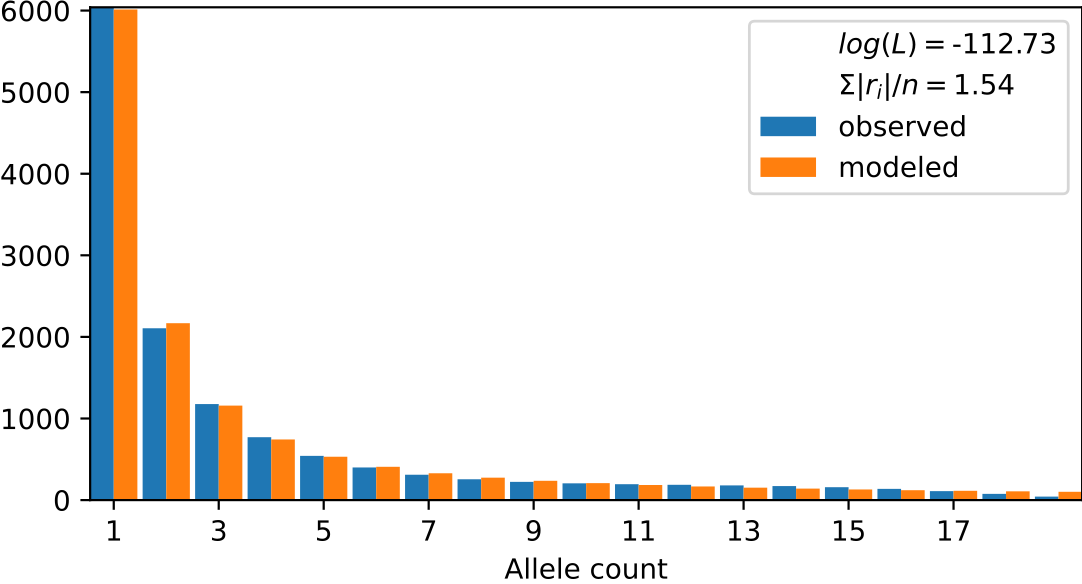
\includegraphics[width=\textwidth]{tetraploid/graphs/png/dadi/one_pop_size_change_since_ice_age/pendula/synonymous/sfs.png}
        \end{subfigure}
        \hfill
        \begin{subfigure}[b]{0.525\textwidth}
            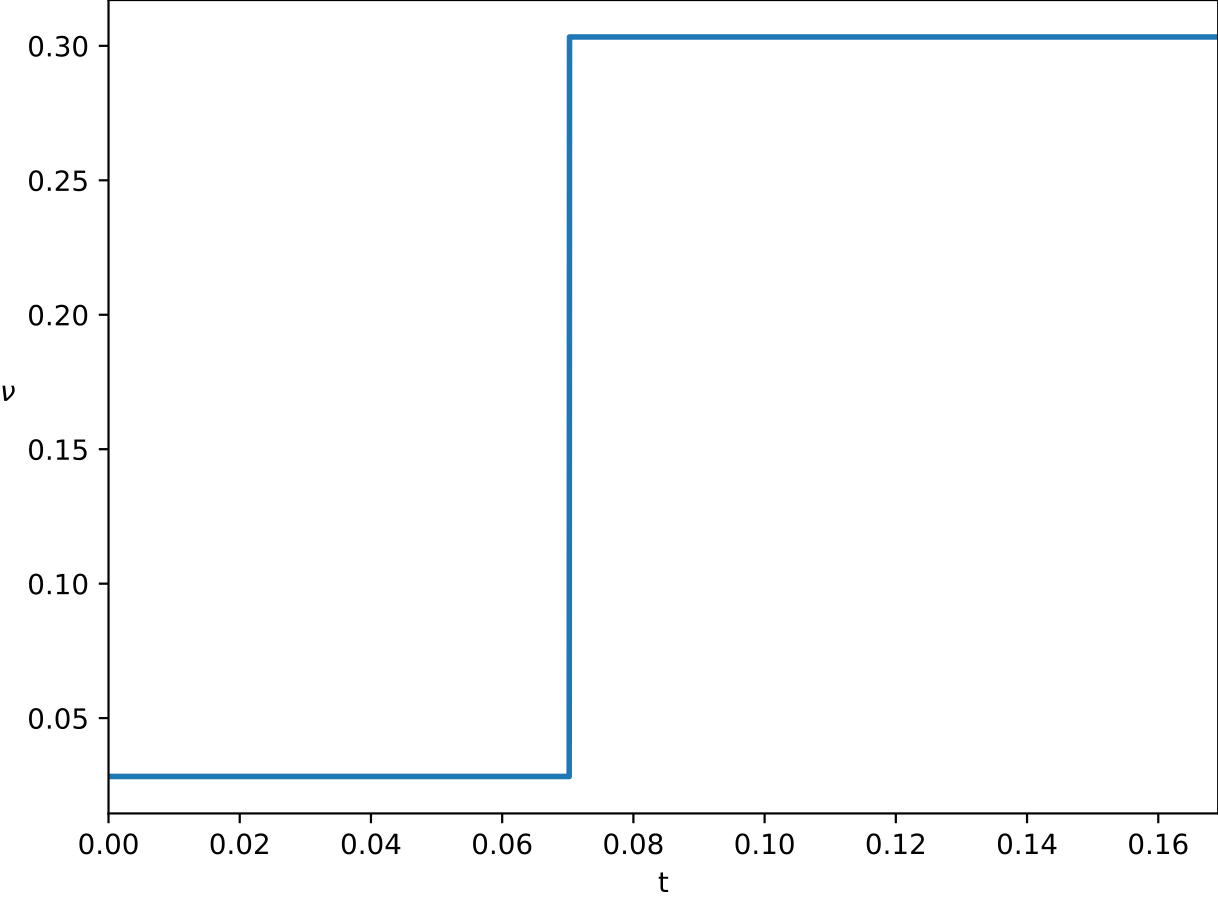
\includegraphics[width=\textwidth]{tetraploid/graphs/png/dadi/one_pop_size_change_since_ice_age/pendula/synonymous/trajectory.png}
        \end{subfigure}
        \caption{One population size change after the \acrshort{lgm} for \pendula{}. This scenario provides the best fit among all tested 1D population scenarios.}
        \label{fig:one_pop_size_change_since_ice_age_pendula}
    \end{figure}

    The one-population models presented here are rather simple but there is not much more that can be included in the absence of selection. None of the models manages to completely capture the excess of high-frequency derived alleles we observe for \pendula{} (cf. figs.~\ref{fig:one_pop_size_change_since_ice_age_pendula} \& \ref{fig:constant_pop_size_since_ice_age_pendula} - \ref{fig:one_pop_size_change_pendula}). This excess could be due to a more fine-scale population structure, ancestral misidentification errors, selection acting directly on synonymous sites or multiple-merger coalescents where some individuals produce disproportionally many offspring. We nevertheless obtain lower average residuals than for \pubescens{} for which we have a deficit of high-frequency derived alleles (cf. figs.~\ref{fig:constant_pop_size_since_ice_age_pubescens} - \ref{fig:one_pop_size_change_pubescens}). In summary, the results indicate population expansion in the not too distant past which is in line with postglacial recolonisation (given that we approximated the time after the \acrshort{lgm} reasonably well). The models were also tested for different fixed time values which suggested similar results. \pubescens{}' estimates may very well be confounded by the signatures of its polyploid ancestors but the results also indicate recent population expansion.

    To confirm our hypothesis about population expansion, Tajima's $D$ was calculated whose values were determined to be -0.95, -1.49 and -1.73 for \pendula{}, \pubescens{} and both species together, respectively. VCFtools was used for the calculations, specifying a window size of 1000 bps from which a weighted average was calculated (cf. fig.~\ref{fig:tajimas_d} for frequency distributions). Inferring Tajima's $D$ from the \acrshort{sfs} using \dadi{} provided values of -1.36, -1.79 and -1.92 which are consistently lower and should be less biased as \pubescens{}'s proper ploidy could be used. Negative values of Tajima's $D$ are common in practice, but could, in principle, be indicative of population expansion. They are, however, well within the margins of the basic coalescent's expectations \cite{hein,gillespie}.

    \subsection{Two-Population Scenarios}

    Modelling scenarios involving two populations, we can include migration which causes the site-wise allele frequencies of the populations to be correlated. Migration cannot so easily be confounded with other dynamics as the only other explanation for correlated allele frequencies is a common origin or an extremely similar demography. It is, however, more difficult to know when migration occurred and at which intensity. Intuitively, extensive recent admixture can have a similar signature to more moderate admixture further in the past. Table~\ref{tbl:2d_dadi} displays parameter estimates for several 2D scenarios involving migration between \pendula{} and \pubescens{}. Here we consider different types of migration and possibly include population growth. Modelling migration between the southern and northern subpopulations of each species continuously hit the upper migration rate boundaries (cf. table~\ref{tbl:param_bounds}). High rates being computationally very expensive, no attempts were made to estimate them further. Some \acrshort{mle} estimates for $t$ are close to their upper bound ($\nu_{up} = 1$) but we found estimates for larger values of $\nu_{up}$ to be quite similar.

    \begin{table}[H]
        \begin{center}
            \resizebox{\textwidth}{!}{
                \setlength\tabcolsep{6pt}
                \begin{tabular}{|l|l|l|l|l|l|l|l|}
                    scenario                            & $log(L)$         & $t$                           & $\nu_{pub}$                        & $\nu_{pen}$              & $m_{pen \rightarrow pub}$    & $m_{pub \rightarrow pen}$    \\
                    $\text{migr}_{none}$                & -2260\,$\pm$\,89 & 0.24\,$\pm$\,0.0083           & 4.9\,$\pm$\,0.21                   & 0.43\,$\pm$\,0.023 & 0                   & 0                    \\
                    $\text{migr}_{pen \rightarrow pub}$ & -1371\,$\pm$\,51 & 0.95\,$\pm$\,0.047            & 3.2\,$\pm$\,0.14 & 0.78\,$\pm$\,0.038 & 1.3\phantom{0}\,$\pm$\,0.06 & 0 \\
                    $\text{migr}_{pub \rightarrow pen}$ & -1995\,$\pm$\,80 & 0.4\phantom{0}\,$\pm$\,0.024   & 4.5\,$\pm$\,0.15 & 0.35\,$\pm$\,0.017 & 0 & 1.1\phantom{0}\,$\pm$\,0.069 \\
                    $\text{migr}_{sym}$                 & -1435\,$\pm$\,58 & 0.9\phantom{0}\,$\pm$\,0.05   & 4.0\,$\pm$\,0.19          & 0.47\,$\pm$\,0.028 & 0.69\,$\pm$\,0.035                   & 0.69\,$\pm$\,0.035                    \\
                    $\text{migr}_{asym}$                & -1280\,$\pm$\,50 & 1.0\phantom{0}\,$\pm$\,0.0044 & 3.3\,$\pm$\,0.13          & 0.65\,$\pm$\,0.02 & 1.1\phantom{0}\,$\pm$\,0.045 & 0.22\,$\pm$\,0.019 \\
                    $\text{migr}_{sym}$\,+\,growth      & -1227\,$\pm$\,46 & 0.82\,$\pm$\,0.058            & 3.2\phantom{0}\,$\rightarrow$\,1.4                & 0.19\,$\rightarrow$\,3.5 & 0.73\,$\pm$\,0.033                   & 0.73\,$\pm$\,0.033                     \\
                    $\text{migr}_{asym}$\,+\,growth     & -1091\,$\pm$\,33 & 0.99\,$\pm$\,0.031            & 0.59\,$\rightarrow$\,6.6                & 0.37\,$\rightarrow$\,2.5  & 1.1\phantom{0}\,$\pm$\,0.037 & 0.31\,$\pm$\,0.016 \\
                \end{tabular}}
        \end{center}
        \caption{2D migration scenarios. Parameters $\nu_{pub}$ and $\nu_{pen}$ denote the relative population size of \pubescens{} and \pendula{}, respectively. Migration from \pendula{} to \pubescens{} is denoted by $m_{pen \rightarrow pub}$ and vice versa. The subscripts $sym$, $asym$ and $none$ denote symmetric, asymmetric and no migration, respectively. Population growth is modelled by a single discrete population size change. Everything takes place during time $t$ and $log(L)$ denotes the log-likelihood. For the scenarios including growth we write $\nu_0 \rightarrow \nu_t$ for the values of $\nu$ at time 0 and $t$. The standard deviation has again been calculated from 100 \acrfull{bca} bootstraps and the point estimates are the average values thereof.}
        \label{tbl:2d_dadi}
    \end{table}

    Migration from \pendula{} into \pubescens{} is consistently estimated to be higher than vice versa which agrees with the expectations about polyploid introgression (cf. section \ref{sec:species}). Figs.~\ref{fig:dadi_2d_residuals_growth_variable_time}, \ref{fig:dadi_2d_residuals_constant_size_variable_time} \& \ref{fig:dadi_2d_residuals_variable_time_migration_constant_size} visualise the residuals for some of the models. The most complex model--asymmetric migration with population growth--provides the highest likelihood (cf. fig.~\ref{fig:dadi_sfs_best_fixed_time_model}). P-value comparisons for the nested models in table~\ref{tbl:2d_dadi} as well as for fixed vs variable-time models can be found in the appendix (cf. fig.~\ref{fig:nested_models_2d}). Similar to the one-population case for \pubescens{}, we obtain significantly lower likelihoods when trying to fix the time to the end of the \acrshort{lgm} (cf. figs.~\ref{fig:dadi_2d_residuals_no_migration_fixed_time} - \ref{fig:dadi_2d_residuals_growth_fixed_time} and p-values in fig.~\ref{fig:nested_models_2d_lgm}). This is again due the very short time span integrated over.

    \begin{figure}[H]
        \centering
        \begin{subfigure}[b]{0.48\textwidth}
            \includegraphics[width=\textwidth]{tetraploid/graphs/png/dadi/split_symmetric_migration_one_pop_size_change/pendula_pubescens/synonymous/residuals.png}
            \caption{sym. migration + 1-size change}
        \end{subfigure}
        \hfill
        \begin{subfigure}[b]{0.503\textwidth}
            \includegraphics[width=\textwidth]{tetraploid/graphs/png/dadi/split_asymmetric_migration_one_pop_size_change/pendula_pubescens/synonymous/residuals.png}
            \caption{asym. migration + 1-size change\label{fig:dadi_2d_residuals_asymmetric_growth_variable_time}}
        \end{subfigure}
        \caption{Anscombe residuals for 2D scenarios with \mbox{(a)-symmetric} migration and population growth over variable time. These scenarios are the most complex ones and achieve higher likelihoods than all other models. The observed and modelled \acrshort{sfs} of (\subref{fig:dadi_2d_residuals_asymmetric_growth_variable_time}) are shown in fig.~\ref{fig:dadi_sfs_best_fixed_time_model}.}
        \label{fig:dadi_2d_residuals_growth_variable_time}
    \end{figure}

    \subsection{Discussion}

    The demographic analyses mostly confirmed our expectations on recent population expansion and asymmetric gene flow between the two species. The lack of precise parameter estimate for $N_e$ and $\mu$ make more precise inferences difficult within this framework. Coalescent simulations could shed light on more fine-scale population structure or more detailed population size trajectories but the problem of $N_e$ remains. Having more precise trajectories, one might be able to discern several glaciations. The models also support gene flow from \pubescens{} to \pendula{}, although at lower rates which is not implausible. In fact, there has also been found to be bi-directional gene flow between \pubescens{} and \nana{} in Iceland \cite{birch-hybridisation-nana-pubescens}.

    \clearpage


    \section{The Distribution of Fitness Effects}
    \label{sec:dfe}

    In section \ref{sec:degeneracy-synonymy}, we already mentioned that most non-synonymous mutations are deleterious. This makes sense intuitively for coding sites considering that a protein with its extremely fine-tuned structure will most likely perform worse when randomly changing one of its amino acids. If we are interested in how likely a novel mutation modifies the carrier's fitness by a certain amount, we are led to the concept of the \acrfull{dfe} which is simply a frequency distribution of selection coefficients for derived genetic variants. The \acrshort{dfe} can be either determined empirically by conducting mutagenesis experiments or theoretically by inferring it from polymorphism data. Knowing the \acrshort{dfe} of a certain organism can help resolve an array of important questions regarding the accumulation of deleterious mutations or the nature of quantitative traits \cite{dfe-review}.

    \subsection{Methods}

    \begin{figure}[ht]
        \centering
        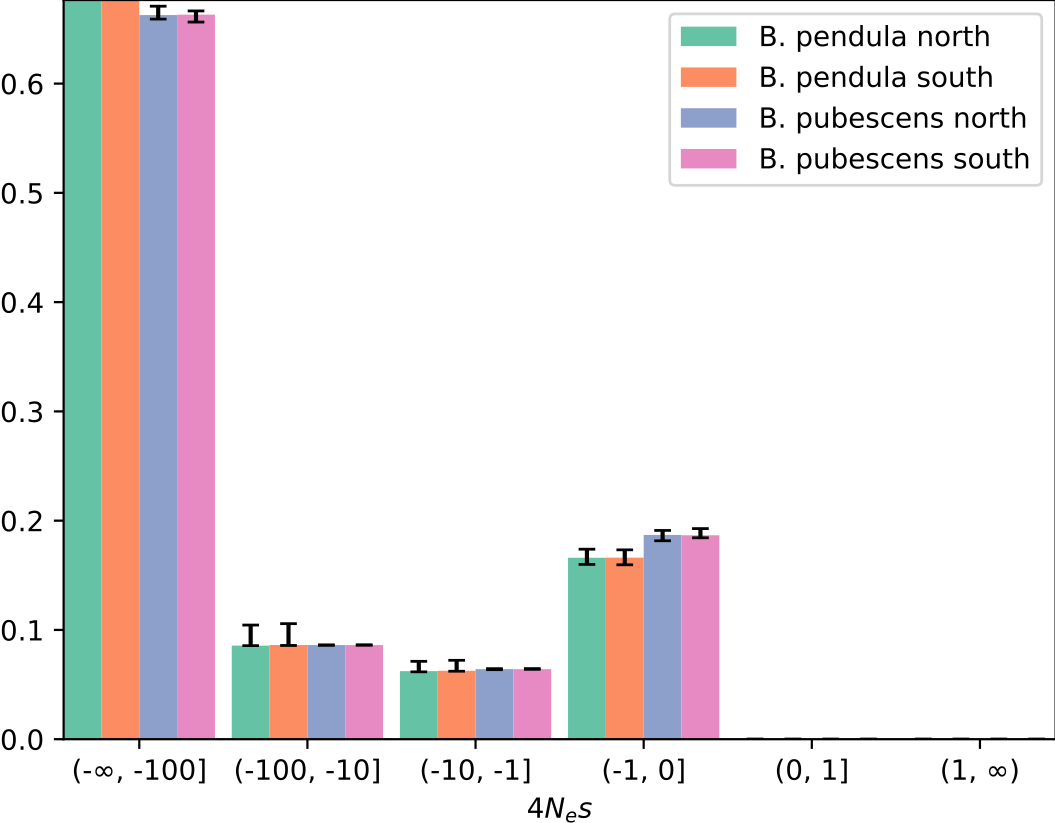
\includegraphics[width=0.9\textwidth]{tetraploid/graphs/png/polydfe/dfe_subpopulations_bs_bca.C.deleterious_anc.png}
        \caption{The deleterious \acrshort{dfe} for the four different subpopulations. The shape is remarkably similar between the two species.}
        \label{fig:dfe_subpopulations_deleterious}
    \end{figure}

    We used polyDFE for the inference \cite{polydfe}. As input, an unfolded \acrshort{sfs} for both synonymous and non-synonymous sites is required. The synonymous sites are assumed to be neutrally-evolving, in addition to assuming that demography affects synonymous and non-synonymous sites in the same manner. The difference in the non-synonymous \acrshort{sfs} compared to the synonymous one is thus caused by selection so that we can infer the strength of selection by controlling for all other factors, i.e. demography. A similar principle is put to use in the well-known McDonald-Kreitman test where the ratio of non-synonymous to synonymous polymorphism within a species is compared to the ratio of non-synonymous to synonymous substitutions across species \cite{mk-test}. In polyDFE, however, passing divergence data is optional and was avoided in this analysis. Besides that, we are required to specify the total number of surveyed sites. \acrfull{mle} is again used to find the best fitting parameters with the expected allele frequencies being inferred from Poisson Random Field theory which is diffusion-based. This is similar to how \dadi{} works. Poisson likelihoods are used again, but this time for each site independently (assuming that we do not choose to model variable mutation rates). This is opposed to independent Poisson likelihoods per frequency class in \dadi{}. Nuisance parameters are used to correct for demography, and ancestral misidentification can optionally be included by introducing a single parameter modelling the probability of any site being assigned the wrong ancestral state (cf. fig.~\ref{fig:dfe_type_C_pendula}).

    The \acrshort{dfe}'s default shape is assumed to follow a reflected gamma distribution for non-positive selection coefficients and an exponential distribution for positive ones. This model is used for all displayed \acrshort{dfe}s if not otherwise specified and is polyDFE's default model. Different models and a brief comparison between them can be found in the appendix (cf. figs.~\ref{fig:dfe_type_C} - \ref{fig:dfe_type_A}). The exponential shape for positive selection coefficients, i.e. a much higher probability of slightly advantageous mutations compared to strongly advantageous ones, seems plausible when considering \acrfull{fgm}. That is, if we assume the fitness of an organism to be close to a local maximum as well as being determined by many interdependent parameters (e.g. \acrshort{snp}s), then a large fitness increase by changing only one of the parameter seems unlikely. The distribution for negative selection coefficients is more complex, possibly being multimodal (i.e. having several maxima). This could result from there being several component distributions that overlap \cite{dfe-review}. A gamma distribution, being more flexible and able to assume both the shape of an exponential distribution and a skewed normal-like distribution, is thus more appropriate. In polyDFE, we can also distinguish between estimating only a deleterious \acrshort{dfe}, i.e. only considering negative selection coefficients, and a full \acrshort{dfe} where we also consider beneficial mutations (cf. fig.~\ref{fig:dfe_type_C_pendula}). These models are nested and are thus eligible for model comparison through \acrlong{lrt}s (cf. fig.~\ref{fig:probs_nested}).

    Confidence intervals were determined using 100 \acrfull{bca} bootstraps where the bootstrap samples' allele frequencies were drawn from a Poisson distribution (cf. fig.~\ref{fig:dfe_parameter_dict} for a comparison with percentile bootstraps). The \acrshort{bfgs} algorithm was used which performs local optimisation and is polyDFE's default algorithm. The species' proper ploidies are also reflected properly, the input being \acrshort{sfs}-based.

    \subsection{Results}

    Including ancestral misidentification does not seem to affect the distribution significantly (fig.~\ref{fig:probs_nested_pendula_pubescens} for a p-value comparison for various models). Including advantageous mutations, however, does provide a much better fit which is again apparent in the minute p-values, allowing us to reject the null hypothesis. The significantly larger variance of the effect size and proportion of beneficial mutations visible in fig.~\ref{fig:dfe_type_C_pendula} can be explained by the scarcity of such mutations, having a much smaller impact on the \acrshort{sfs} in comparison to deleterious mutations \cite{dfe-plants}. Strongly advantageous mutations moreover quickly reach fixation, further reducing the number of possible observations \cite{polydfe}.

    A comparison of the \acrshort{dfe} for the two southern and northern subpopulations is shown in figs.~\ref{fig:dfe_subpopulations_deleterious}. There seem to be rather large differences in the number of beneficial mutation between the two species (cf. fig.~\ref{fig:dfe_subpopulations}). \pubescens{} is estimated to have many more slightly advantageous mutations but all confidence intervals, in fact, overlap. This is in contrast with the deleterious \acrshort{dfe}s which have very narrow confidence intervals and are strikingly similar among all subpopulations (cf. fig.~\ref{fig:dfe_subpopulations_deleterious}). For all analyses, the optimisation runs completed with a gradient reasonably small and larger gradients do not seem to introduce a bias to the estimated parameters in general (cf. fig.~\ref{fig:dfe_grad_errors}). Furthermore, the \acrshort{dfe} seems to be rather robust to the bias introduced by calling \pubescens{} as diploid (cf. fig.~\ref{fig:dfe_subpopulation_calling_methods}).

    \subsection{Discussion}

    The strong similarity of the \acrshort{dfe} between the two species is perhaps not that surprising when considering the species' related ancestry. This is especially so, if a species similar to \pendula{} was the autopolyploid ancestor of \pubescens{} (cf. section \ref{sec:expectations}). In a recent paper, the shape of the deleterious \acrshort{dfe} has been found to be very similar across several great ape species  which could be confirmed for the birch species in this work \cite{dfe-similarity-across-species}. Shared ancestry thus seems to be an important determinant in the similarity of the \acrshort{dfe}, the bulk of allele frequencies taking a long time to change after speciation, after all. It can also be argued, however, that closely related species have a rather similar genomic architecture and hence the \acrshort{dfe} is unlikely to change considerably between them. That being said, different species could be subject to environmental pressures of a very different nature and intensity after speciation, which could potentially change the \acrshort{dfe} significantly.

    The full \acrshort{dfe} differs substantially in the amount of beneficial mutations among the two species although the variance in the amount of such mutations is rather high. The amount of beneficial mutations inferred from the \acrshort{sfs} is very sensitive to ancestral misidentification as such mutations are rare and expected to segregate at high frequencies \cite{polydfe}. polyDFE's ancestral misidentification parameter can properly correct for that error provided that the probability of misidentification is the same over all frequency classes which might not be the case, especially when using more elaborate methods for inferring the ancestral states. In the great apes paper, \acrlong{lrt}s did not favour a \acrshort{dfe} including beneficial mutations which, in our case, is true for \pendula{} but not for \pubescens{} (cf. fig.~\ref{fig:probs_nested}). Moreover, the fraction of selectively neutral ($|4N_es| < 1$) or more strongly advantageous ($4N_es \geq 1$) mutations is consistently estimated to be larger in \pubescens{} (compared to \pendula{}) which is in line with a higher value of $\pi_N/\pi_S$ (cf. section \ref{sec:pi}). In all cases, the fraction of such mutations is nevertheless lower than suggested by $\pi_N/\pi_S$ which could be due to the fixation of more strongly deleterious mutations ($4N_es \leq 1$).

    \clearpage


    \section{Closing Words}

    I hope to have provided useful analyses as well as a clear overview of the demography and population structure of \pendula{} and \pubescens{}, two important boreal species, not only to Scandinavia but to large parts of Eurasia as a whole. The polyploid nature of \pubescens{} presented significant obstacles to correct inference but offered, at the same time, many interesting and thought-provoking dynamics. Working with two species in tandem also provided useful comparisons and sanity checks although it was not always immediately apparent where differences stem from. There were also hurdles in the inference of demography, partly because little is known about important parameters like mutation rate, effective population size and generation time. The developed pipeline supplies some useful abstractions to the tools used in this work and will hopefully find repeated use, if only by the author.

    To summarise, this work confirms the existence of a northern and a southern cluster in each species, unidirectional introgression from \pendula{} into \pubescens{}, and population expansion after the \acrshort{lgm}. The \acrshort{dfe} of new mutations between the two species is also remarkably similar and the amount of deleterious mutations seems acceptable. There is thus hope that these species will be able to adapt to future environmental challenges and that \pendula{} continues being a good and sustainable resource for timber. Much remains to be done to unravel the complex interplay and history of these rather flexible species whose prosperity is crucial to a functioning boreal ecosystem.

    \clearpage
    
    \begin{acknowledgements}
        I would like to express my thanks to my supervisor Martin Lascoux for helpful feedback, reading material, personal lectures and a conducive working atmosphere. I would also like to thank my co-supervisor Jennifer James for advising me on potential tools, helping create the project outline and kindly listening to my progress reports. At last, I also owe thanks to Luis Leal for a detailed introduction to the underlying data and useful recommendations.
    \end{acknowledgements}

    \clearpage

    \bibliography{refs}

    \clearpage

	\appendix
	\setcounter{figure}{0}
	\renewcommand{\thefigure}{A\arabic{figure}}

    \section{Appendix}
    \label{sec:appendix}

    \subsection{Pipeline}
    \label{sec:appendix-pipeline}
    
    \begin{figure}[ht]
        \centering
        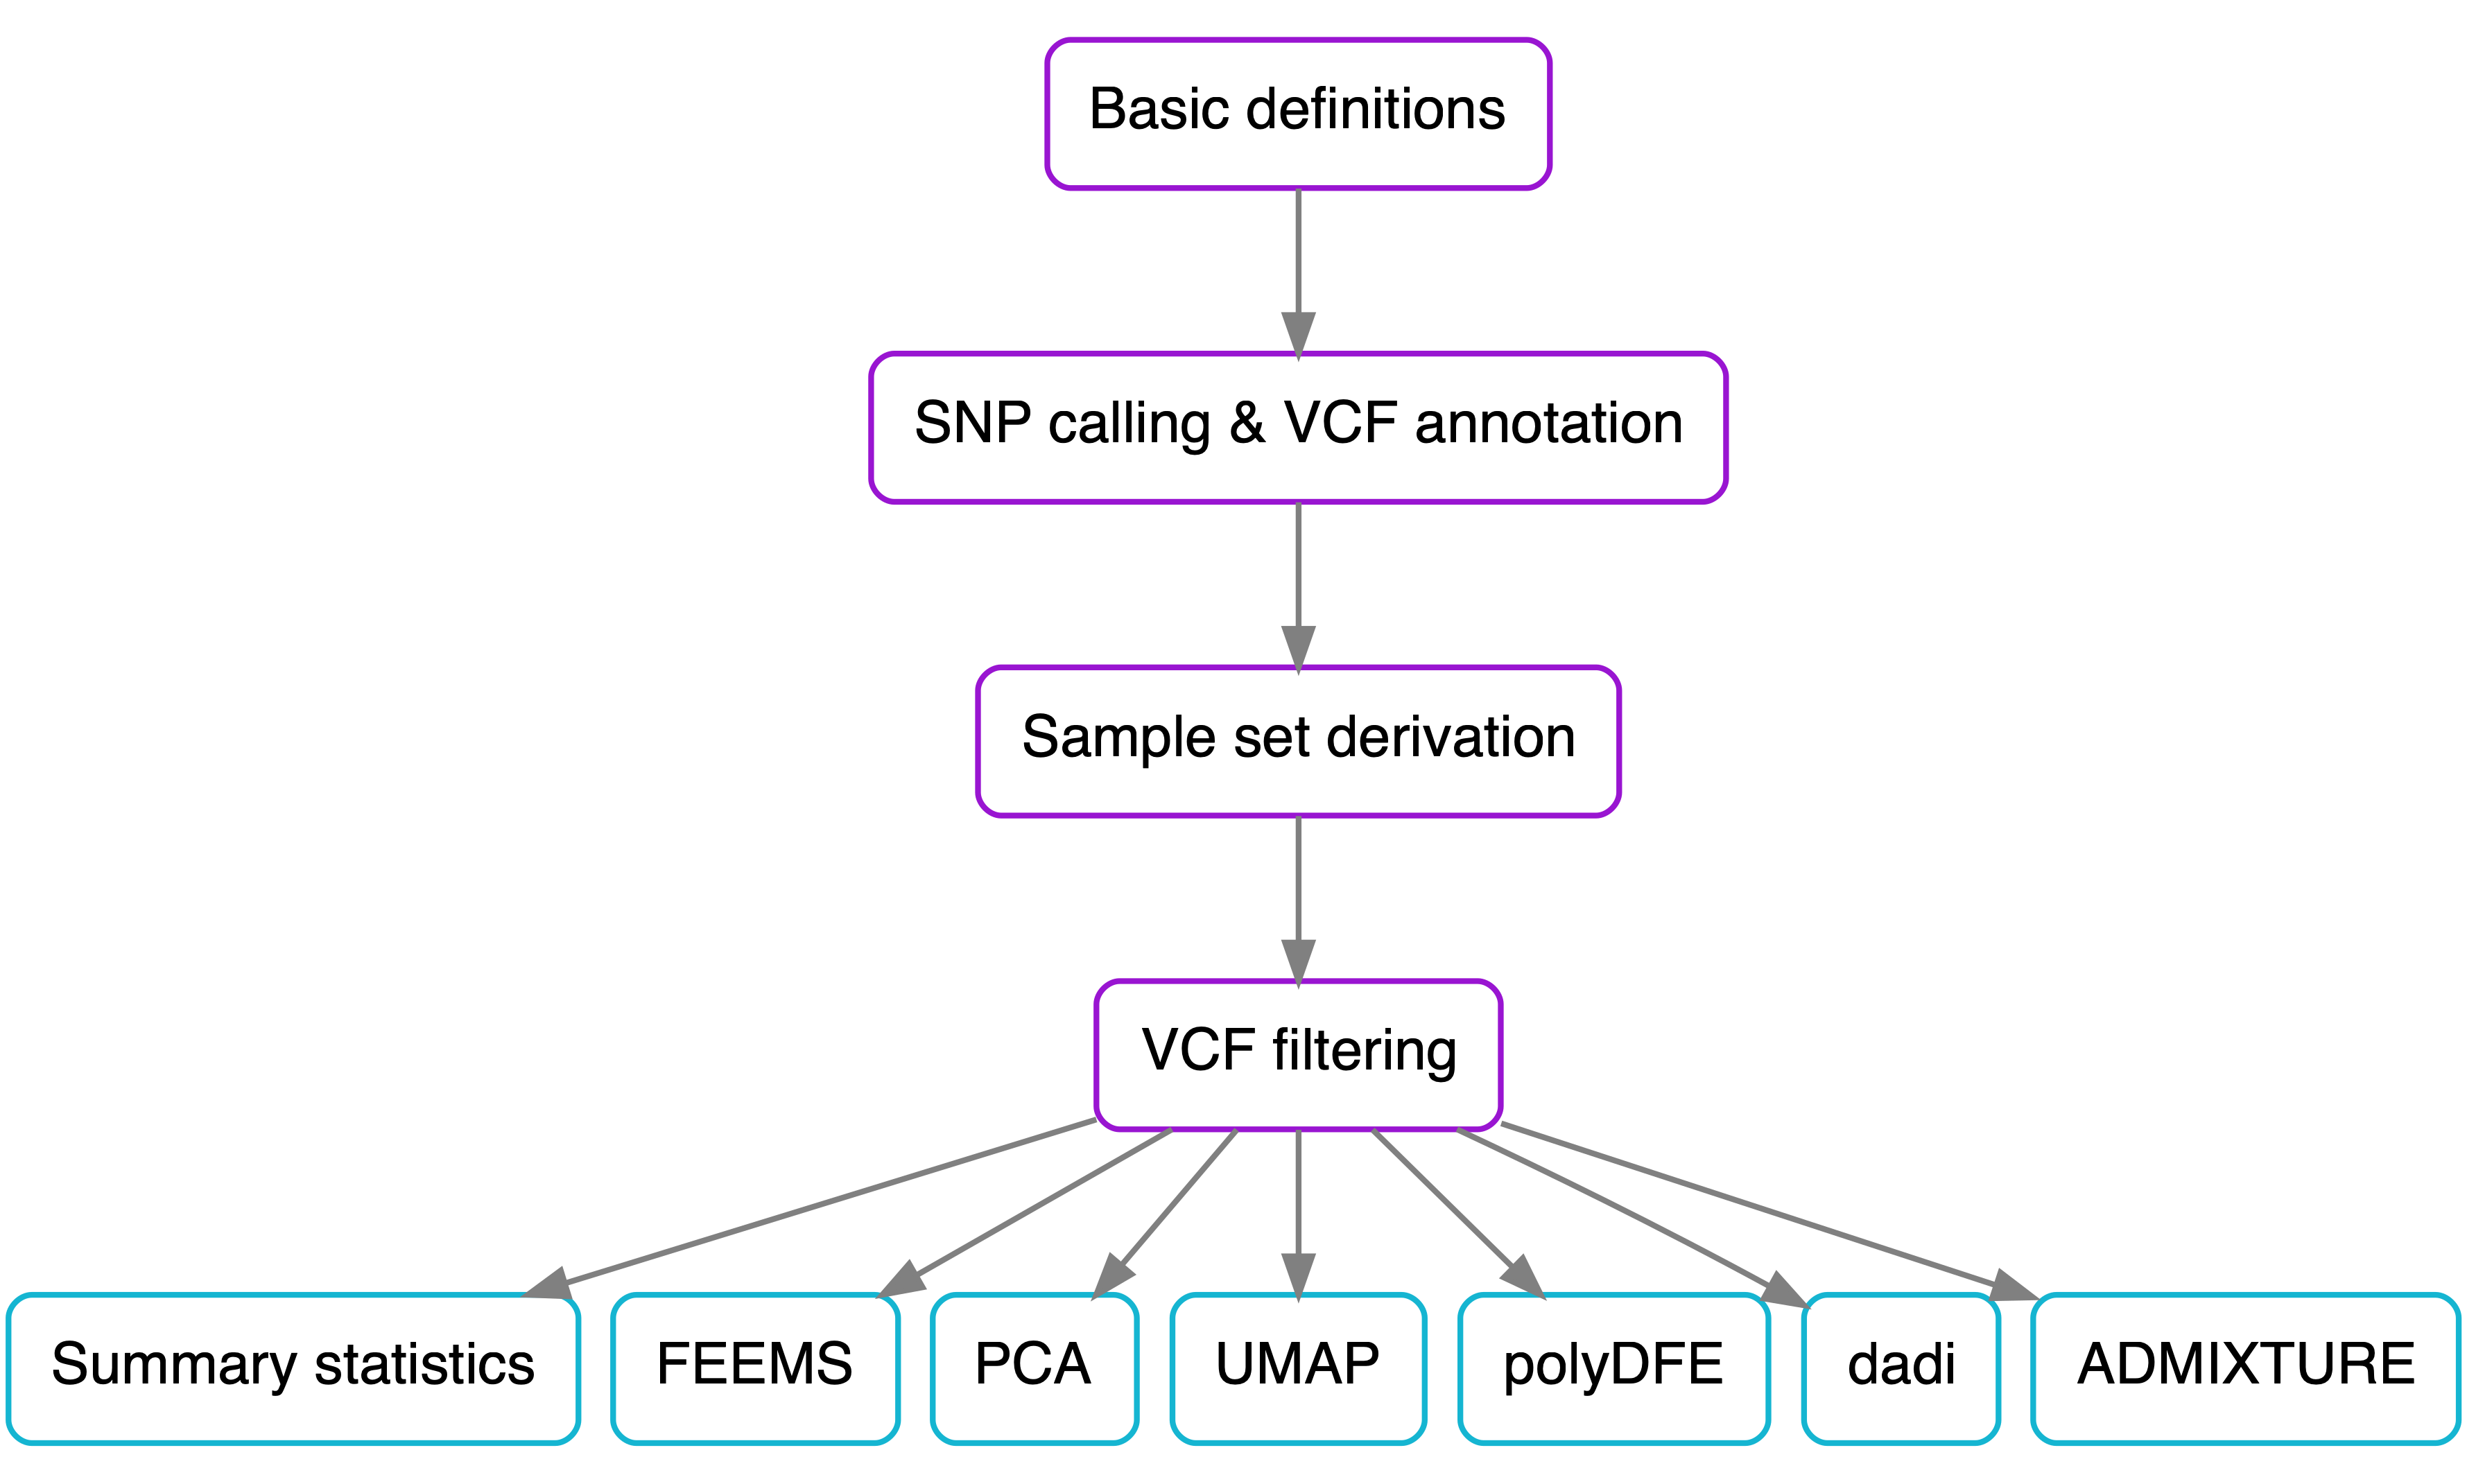
\includegraphics[width=\textwidth]{default/graphs/png/rulegraphs/schematics/subworkflows.png}
        \caption{A schematic of the pipeline's subworkflows. Each subworkflow can be executed independently. The \acrshort{vcf} filtering relies on the previous annotation of the \acrshort{vcf} files as well as the derived sample sets (i.e. which individuals to include). The lowermost subworkflows only require a \acrshort{vcf} file and possibly some sample metadata and subpopulation information.}
        \label{fig:subworkflows}
    \end{figure}

    \begin{figure}[H]
        \centering
        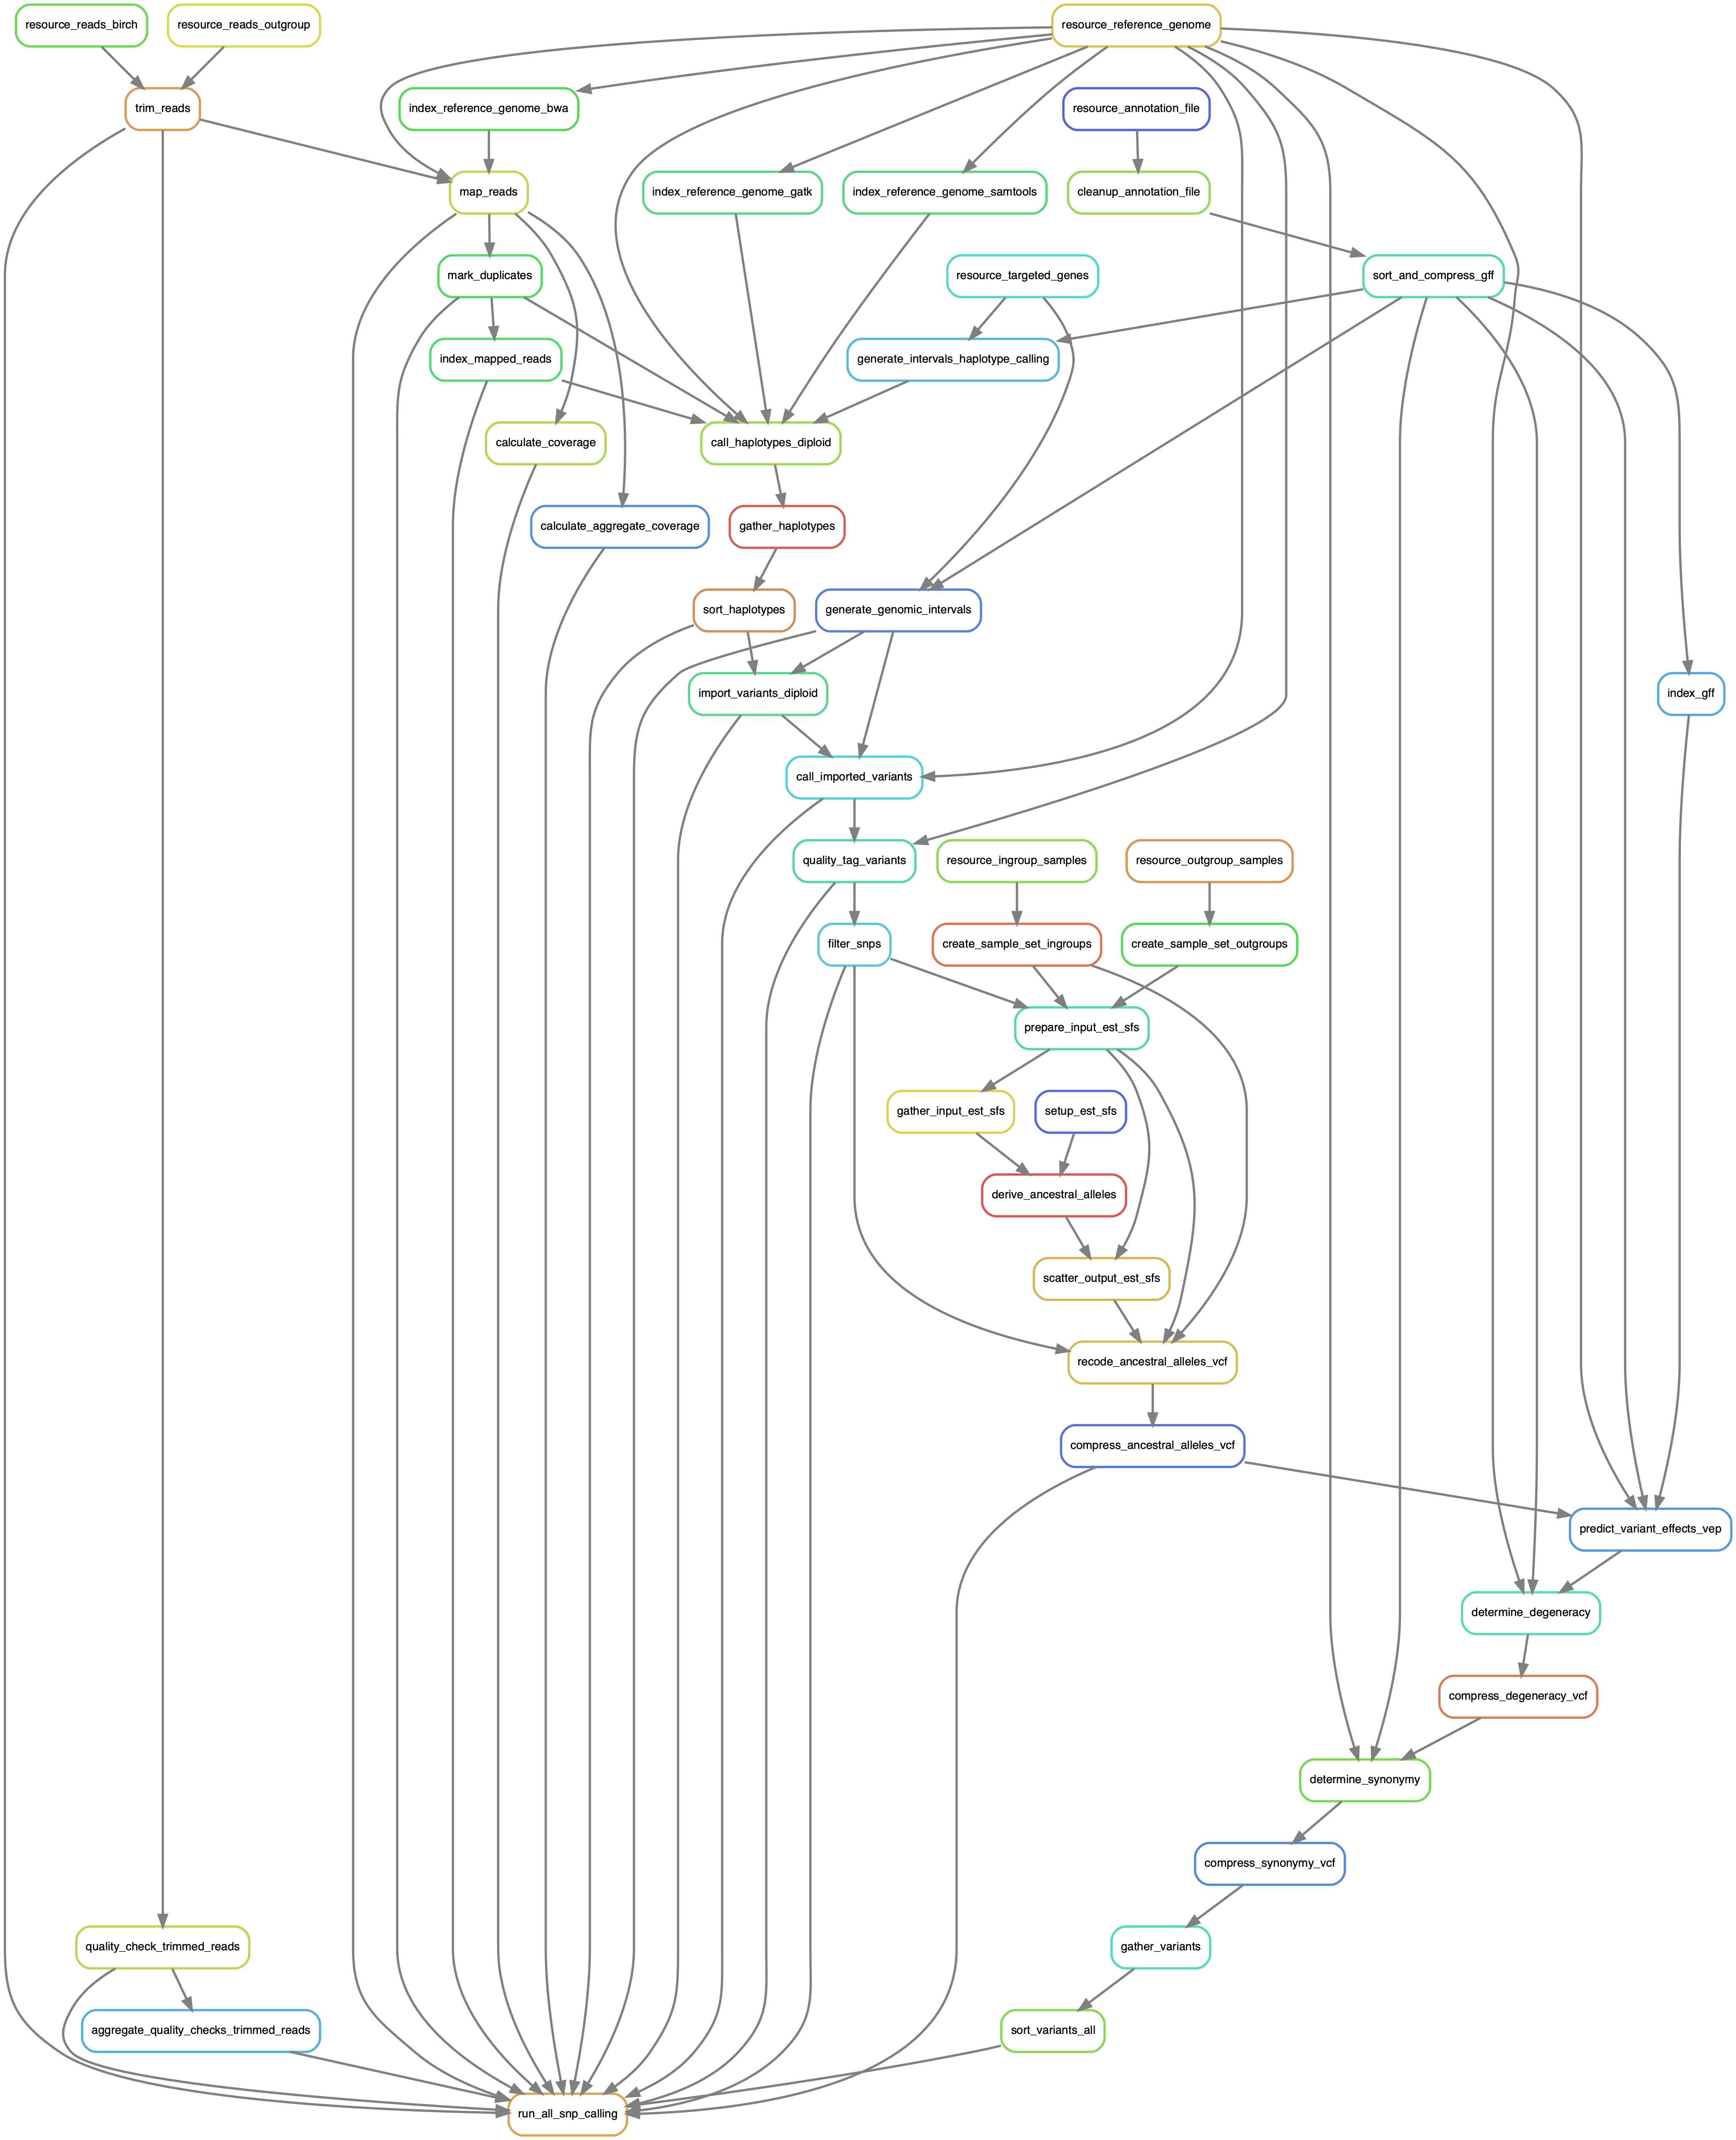
\includegraphics[width=\textwidth]{default/graphs/png/rulegraphs/snp_calling.png}
        \caption{Workflow to obtain the initial \acrshort{vcf} file from the raw reads.}
    \end{figure}

    \clearpage

    \subsection{Summary Statistics}
    \label{sec:basic-stats}

    \subsubsection{$F_{ST}$}

    \begin{figure}[H]
        \centering
        \begin{subfigure}[b]{0.49\textwidth}
            \centering
            \includegraphics[width=\textwidth]{default/graphs/png/fst/pendula/all/fst.log.png}
            \caption{\pendula{}}
        \end{subfigure}
        \hfill
        \begin{subfigure}[b]{0.49\textwidth}
            \centering
            \includegraphics[width=\textwidth]{default/graphs/png/fst/pubescens/all/fst.log.png}
            \caption{\pubescens{}}
        \end{subfigure}
        \caption{Log-scaled frequency distributions for site-wise values of the $F_{ST}$.}
        \label{fig:fst}
    \end{figure}

    \subsubsection{Tajima's D}

    \begin{figure}[H]
        \centering
        \begin{subfigure}[b]{0.49\textwidth}
            \centering
            \includegraphics[width=\textwidth]{default/graphs/png/tajimas_d/pendula/all/tajimas_d.linear.png}
            \caption{\pendula{}}
            \label{fig:tajimas_d_pendula}
        \end{subfigure}
        \hfill
        \begin{subfigure}[b]{0.49\textwidth}
            \centering
            \includegraphics[width=\textwidth]{default/graphs/png/tajimas_d/pubescens/all/tajimas_d.linear.png}
            \caption{\pubescens{}}
            \label{fig:tajimas_d_pubescens}
        \end{subfigure}
        \caption{Frequency distributions for values of Tajima's $D$ with a window size of 1000 bps.}
        \label{fig:tajimas_d}
    \end{figure}

    \subsubsection{Heterozygosity}
    
    \begin{figure}[ht]
        \centering
        \begin{subfigure}[b]{0.485\textwidth}
            \centering
            \includegraphics[width=\textwidth]{default/graphs/png/heterozygosity/pendula/all/het.log.png}
            \caption{\pendula{}}
            \label{fig:het_pendula}
        \end{subfigure}
        \hfill
        \begin{subfigure}[b]{0.485\textwidth}
            \centering
            \includegraphics[width=\textwidth]{default/graphs/png/heterozygosity/pubescens/all/het.log.png}
            \caption{\pubescens{}}
            \label{fig:het_pubescens}
        \end{subfigure}
        \caption{Expected (under \acrshort{hwe}) and observed site-wise heterozygosity over the set of bi- and mono-allelic sites. The observed excess heterozygosity for \pubescens{} is caused by calling it as diploid. The expected site-wise heterozygosity is equivalent to the nucleotide diversity $\pi$. The dashed vertical lines indicate the average heterozygosities. Note that these plots are log-scaled.}
        \label{fig:het}
    \end{figure}

    \begin{figure}[H]
        \centering
        \begin{subfigure}[b]{0.49\textwidth}
            \centering
            \includegraphics[width=\textwidth]{default/graphs/png/heterozygosity/pendula/biallelic/het.linear.png}
            \caption{\pendula{}}
            \label{fig:het_linear_pendula}
        \end{subfigure}
        \hfill
        \begin{subfigure}[b]{0.49\textwidth}
            \centering
            \includegraphics[width=\textwidth]{default/graphs/png/heterozygosity/pubescens/biallelic/het.linear.png}
            \caption{\pubescens{}}
            \label{fig:het_linear_pubescens}
        \end{subfigure}
        \caption{Linearly scaled plots of the expected and observed heterozygosity on the set of bi-allelic sites. }
        \label{fig:het_linear}
    \end{figure}

    \begin{figure}[H]
        \centering
        \begin{subfigure}[b]{0.49\textwidth}
            \centering
            \includegraphics[width=\textwidth]{default/graphs/png/hwe/pendula/all/p.log.png}
            \caption{\pendula{}}
            \label{fig:p_hwe_pendula}
        \end{subfigure}
        \hfill
        \begin{subfigure}[b]{0.49\textwidth}
            \centering
            \includegraphics[width=\textwidth]{default/graphs/png/hwe/pubescens/all/p.log.png}
            \caption{\pubescens{}}
            \label{fig:p_hwe_pubescens}
        \end{subfigure}
        \caption{Site-wise p-values for observed heterozygosity under \acrshort{hwe}. The two plots and their average p-value are only partly comparable, however, as they depend on the total number of \acrshort{snp}s and their frequencies. Almost all sites are either monomorphic for which we obtain a p-value of 1, or have alleles that segregate far from non-intermediate frequencies for which p-values of 1 are very likely since there is little statistical power to detect deviations from \acrshort{hwe}.}
        \label{fig:p_hwe}
    \end{figure}

    \begin{figure}[H]
        \centering
        \begin{subfigure}[b]{0.49\textwidth}
            \centering
            \includegraphics[width=\textwidth]{default/graphs/png/hwe/pendula/all/midp.log.png}
            \caption{\pendula{}}
        \end{subfigure}
        \hfill
        \begin{subfigure}[b]{0.49\textwidth}
            \centering
            \includegraphics[width=\textwidth]{default/graphs/png/hwe/pubescens/all/midp.log.png}
            \caption{\pubescens{}}
        \end{subfigure}
        \caption{Mid-p-values for heterozygosity under \acrshort{hwe}.}
        \label{fig:mid-p-hwe}
    \end{figure}

    \subsubsection{Missingness}

    \begin{figure}[H]
        \centering
        \begin{subfigure}[b]{0.49\textwidth}
            \centering
            \includegraphics[width=\textwidth]{default/graphs/png/missingness/pendula/all/missingness.l.log.png}
            \caption{\pendula{}}
        \end{subfigure}
        \hfill
        \begin{subfigure}[b]{0.49\textwidth}
            \centering
            \includegraphics[width=\textwidth]{default/graphs/png/missingness//pubescens/all/missingness.l.log.png}
            \caption{\pubescens{}}
        \end{subfigure}
        \caption{Missingness per site.}
        \label{fig:missingness-sample}
    \end{figure}

    \begin{figure}[H]
        \centering
        \begin{subfigure}[b]{0.49\textwidth}
            \centering
            \includegraphics[width=\textwidth]{default/graphs/png/missingness/pendula/all/missingness.i.log.png}
            \caption{\pendula{}}
        \end{subfigure}
        \hfill
        \begin{subfigure}[b]{0.49\textwidth}
            \centering
            \includegraphics[width=\textwidth]{default/graphs/png/missingness/pubescens/all/missingness.i.log.png}
            \caption{\pubescens{}}
        \end{subfigure}
        \caption{Missingness per individual.}
        \label{fig:missingness-individual}
    \end{figure}

    \clearpage

    \subsection{PCA}
    \label{sec:appendix-pca}

    \begin{figure}[H]
        \centering
        \begin{subfigure}[b]{0.49\textwidth}
            \centering
            \includegraphics[width=\textwidth]{default/graphs/png/pca/pendula/biallelic/pca_tight_layout.png}
            \caption{\pendula{}}
            \label{fig:pca_pendula}
        \end{subfigure}
        \hfill
        \begin{subfigure}[b]{0.501\textwidth}
            \centering
            \includegraphics[width=\textwidth]{default/graphs/png/pca/pubescens/biallelic/pca_tight_layout.png}
            \caption{\pubescens{}}
            \label{fig:pca_pubescens}
        \end{subfigure}
        \caption{\acrshort{pca} plots on the set of bi-allelic sites. There are two outliers in the \acrshort{pca} plot for \pendula{} which are not apparent in the plot for synonymous sites (cf. fig.~\ref{fig:pca_synonymous_pendula}).}
        \label{fig:pca_pendula_pubescens_separate}
    \end{figure}

    \begin{figure}[H]
        \centering
        \begin{subfigure}[b]{0.493\textwidth}
            \centering
            \includegraphics[width=\textwidth]{default/graphs/png/pca/pendula/nonsynonymous/pca_tight_layout.png}
            \caption{\pendula{}}
            \label{fig:pca_nonsynonymous_pendula}
        \end{subfigure}
        \hfill
        \begin{subfigure}[b]{0.49\textwidth}
            \centering
            \includegraphics[width=\textwidth]{default/graphs/png/pca/pubescens/nonsynonymous/pca_tight_layout.png}
            \caption{\pubescens{}}
            \label{fig:pca_nonsynonymous_pubescens}
        \end{subfigure}
        \caption{\acrshort{pca} plots on the set of non-synonymous sites. The rather weak population structure of \pendula{} is not apparent at all in this case (cf. fig.~\ref{fig:pca_pendula}).}
        \label{fig:pca_pendula_pubescens_separate_nonsynonymous}
    \end{figure}

    \clearpage

    \subsection{UMAP}
    \label{sec:appendix-umap}

    \begin{figure}[H]
        \centering
        \begin{subfigure}[b]{0.487\textwidth}
            \centering
            \includegraphics[width=\textwidth]{default/graphs/png/umap/pendula/biallelic/umap_tight_layout.png}
            \caption{\pendula{}}
            \label{fig:umap_biallelic_pendula}
        \end{subfigure}
        \hfill
        \begin{subfigure}[b]{0.5\textwidth}
            \centering
            \includegraphics[width=\textwidth]{default/graphs/png/umap/pubescens/biallelic/umap_tight_layout.png}
            \caption{\pubescens{}}
            \label{fig:umap_biallelic_pubescens}
        \end{subfigure}
        \caption{\acrshort{umap} plots on the set of bi-allelic sites for each of the two birch species. The \texttt{spread} and \texttt{min\_dist} parameters were set to 2 and 0, respectively.}
        \label{fig:umap_biallelic_pendula_pubescens_separate}
    \end{figure}

    \clearpage

    \subsection{ADMIXTURE}

    \begin{figure}[H]
        \centering
        \begin{subfigure}[b]{0.313\textwidth}
            \centering
            \includegraphics[width=\textwidth]{default/graphs/png/admixture/pendula/biallelic/cv_error.4.png}
            \caption{\pendula{}}
            \label{fig:admixture_cv_error_pendula}
        \end{subfigure}
        \hfill
        \begin{subfigure}[b]{0.32\textwidth}
            \centering
            \includegraphics[width=\textwidth]{default/graphs/png/admixture/pubescens/biallelic/cv_error.4.png}
            \caption{\pubescens{}}
            \label{fig:admixture_cv_error_pubescens}
        \end{subfigure}
        \hfill
        \begin{subfigure}[b]{0.32\textwidth}
            \centering
            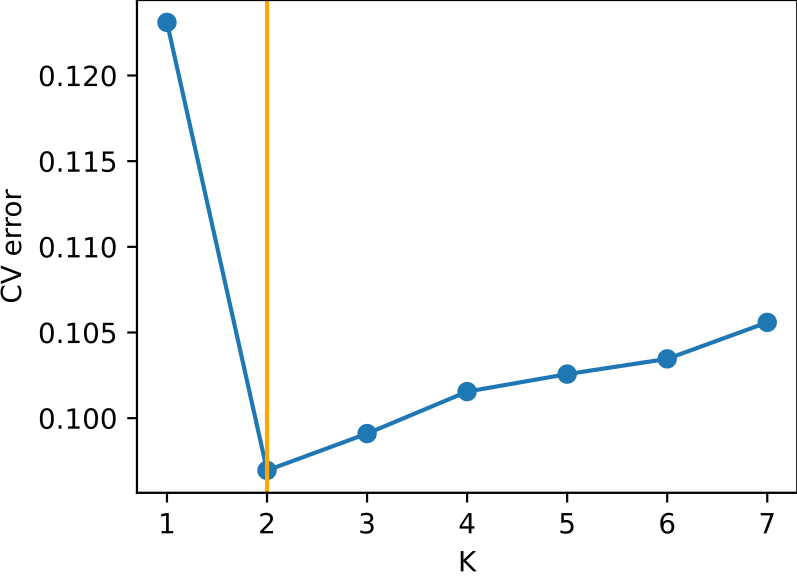
\includegraphics[width=\textwidth]{default/graphs/png/admixture/pendula_pubescens/biallelic/cv_error.7.png}
            \caption{both species}
            \label{fig:admixture_cv_error_both_species}
        \end{subfigure}
        \caption{5-fold cross validation error over the number of clusters $K$. A single population ($K=1$) is erroneously favoured within each of the two species. The set of bi-allelic sites was used for all analyses.}
        \label{fig:admixture_cv_error_pendula_pubescens}
    \end{figure}
    
    \begin{figure}[H]
        \centering
        \begin{subfigure}[b]{0.306\textwidth}
            \centering
            \includegraphics[width=\textwidth]{default/graphs/png/admixture/pendula/biallelic/locations.png}
            \caption{\pendula{}}
            \label{fig:locations_admixture_pendula}
        \end{subfigure}
        \hfill
        \begin{subfigure}[b]{0.32\textwidth}
            \centering
            \includegraphics[width=\textwidth]{default/graphs/png/admixture/pubescens/biallelic/locations.png}
            \caption{\pubescens{}}
            \label{fig:locations_admixture_pubescens}
        \end{subfigure}
        \hfill
        \begin{subfigure}[b]{0.32\textwidth}
            \centering
            \includegraphics[width=\textwidth]{default/graphs/png/admixture/pendula_pubescens/biallelic/locations.png}
            \caption{both species}
            \label{fig:locations_admixture_pendula_pubescens}
        \end{subfigure}
        \caption{Jittered sample locations labeled with the \mbox{ADMIXTURE} clustering for $K=2$. The population structure closely resembles the one deduced from the \acrshort{pca} plots.}
        \label{fig:locations_admixture}
    \end{figure}

    \begin{figure}[H]
        \centering
        \begin{subfigure}[b]{0.32\textwidth}
            \centering
            \includegraphics[width=\textwidth]{default/graphs/png/admixture/pendula/biallelic/synonymous/pca.png}
            \caption{\pendula{}}
            \label{fig:pca_admixture_pendula}
        \end{subfigure}
        \hfill
        \begin{subfigure}[b]{0.32\textwidth}
            \centering
            \includegraphics[width=\textwidth]{default/graphs/png/admixture/pubescens/biallelic/synonymous/pca.png}
            \caption{\pubescens{}}
            \label{fig:pca_admixture_pubescens}
        \end{subfigure}
        \hfill
        \begin{subfigure}[b]{0.32\textwidth}
            \centering
            \includegraphics[width=\textwidth]{default/graphs/png/admixture/pendula_pubescens/biallelic/synonymous/pca.png}
            \caption{both species}
            \label{fig:pca_admixture_pendula_pubescens}
        \end{subfigure}
        \caption{\acrshort{pca} scatterplots labeled with the \mbox{ADMIXTURE} clustering for $K=2$. A clustering very similar to the latitudinal gradients in figs.~\ref{fig:pca} \& \ref{fig:pca} is apparent.}
        \label{fig:pca_admixture}
    \end{figure}

    \subsubsection{\pendula{} \& \pubescens{}}
    
    All bar plots are first sorted by the displayed (\mbox{ADMIXTURE}) subpopulations and second by latitude in ascending order.

    \begin{figure}[H]
        \centering
        \includegraphics[width=\textwidth]{default/graphs/png/admixture/pendula_pubescens/biallelic/barplot.3.4.png}
        \caption{Bar plot for both species using $K=3$. Compared to the two-cluster case we now additionally distinguish between a northern and a southern subpopulation for \pubescens{}. \pendula{}'s subpopulation structure is considerably weaker so detecting \pubescens{}'s subpopulation structure first seems reasonable.}
        \label{fig:admixture_barplot_pendula_pubescens_3}
    \end{figure}

    \begin{figure}[H]
        \centering
        \includegraphics[width=\textwidth]{default/graphs/png/admixture/pendula_pubescens/biallelic/barplot.4.4.png}
        \caption{Bar plot for both species using $K=4$. \mbox{ADMIXTURE} further partitions \pubescens{} individuals but compared to $K=3$, no latitudinal structure is apparent. This trend persists for higher values of $K$. The subpopulation structure of \pendula{} is too weak to be detected considering both species together.}
        \label{fig:admixture_barplot_pendula_pubescens_4}
    \end{figure}

    \subsubsection{\pendula{}}

    \begin{figure}[H]
        \centering
        \includegraphics[width=\textwidth]{default/graphs/png/admixture/pendula/biallelic/barplot.2.2.png}
        \caption{Bar plot for \pendula{} using $K=2$. The northern and southern subpopulation are clearly identified. There also seems to be considerable admixture between the two subpopulations, particularly from the northern population into the southern one.}
        \label{fig:admixture_barplot_pendula_2}
    \end{figure}

    \begin{figure}[H]
        \centering
        \includegraphics[width=\textwidth]{default/graphs/png/admixture/pendula/biallelic/barplot.3.2.png}
        \caption{Bar plot for \pendula{} using $K=3$. A third subpopulation is roughly superimposed on the case for $K=2$. This subpopulation does not seem to correlate with latitude, however. For higher values of $K$, we obtain even more scrambled images.}
        \label{fig:admixture_barplot_pendula_3}
    \end{figure}

    \subsubsection{\pubescens{}}

    \begin{figure}[H]
        \centering
        \includegraphics[width=\textwidth]{default/graphs/png/admixture/pubescens/biallelic/barplot.2.2.png}
        \caption{Bar plot for \pubescens{} using $K=2$. The northern and southern subpopulations are clearly identified with considerable admixture being apparent, especially near their contact zone.}
        \label{fig:admixture_barplot_pubescens_2}
    \end{figure}

    \begin{figure}[H]
        \centering
        \includegraphics[width=\textwidth]{default/graphs/png/admixture/pubescens/biallelic/barplot.3.2.png}
        \caption{Bar plot for \pubescens{} using $K=3$. The southern population is now divided into two clusters which do not seem to correlate with latitude, however. For higher values of $K$, we obtain even more disordered images.}
        \label{fig:admixture_barplot_pubescens_3}
    \end{figure}

    \clearpage

    \subsection{FEEMS}
    \label{sec:appendix-feems}

    \subsubsection{1\% cut-off}

    In this subsection, alleles with a frequency lower than 1\% have been removed. A buffer size of 1 was used if not otherwise specified.

    \begin{figure}[H]
        \centering
        \begin{subfigure}[b]{0.48\textwidth}
            \centering
            \includegraphics[width=\textwidth]{default/graphs/png/feems/pendula/no_very_low_freqs/cv_error_warm_start_buffer_1.png}
            \caption{\pendula{}}
        \end{subfigure}
        \hfill
        \begin{subfigure}[b]{0.48\textwidth}
            \centering
            \includegraphics[width=\textwidth]{default/graphs/png/feems/pubescens/no_very_low_freqs/cv_error_warm_start_buffer_1.png}
            \caption{\pubescens{}}
        \end{subfigure}
        \caption{Cross validation error over the smoothing parameter $\lambda$ using warm starts. We obtain similar values of $\lambda$ using cold starts, although with increased variance.}
        \label{fig:feems_cv_error_no_very_low_freqs}
    \end{figure}

    \begin{figure}[H]
        \centering
        \begin{subfigure}[b]{0.47\textwidth}
            \centering
            \frame{\includegraphics[width=\textwidth,height=17em]{default/graphs/png/feems/pendula/no_very_low_freqs/migration_surfaces_cv_buffer_1.png}}
            \caption{\pendula{}}
        \end{subfigure}
        \hfill
        \begin{subfigure}[b]{0.47\textwidth}
            \centering
            \frame{\includegraphics[width=\textwidth,height=17em]{default/graphs/png/feems/pubescens/no_very_low_freqs/migration_surfaces_cv_buffer_1.png}}
            \caption{\pubescens{}}
        \end{subfigure}
        \caption{Migration surface plots for $\lambda$ values of $10$ and $e^{-7}$ for \pendula{} and \pubescens{}, respectively which provided the lowest cross validation error (cf. fig.~\ref{fig:feems_cv_error_no_very_low_freqs}). The right plot seems highly overfitted.}
        \label{fig:feems_no_very_low_freqs_lambda_cv}
    \end{figure}

    \begin{figure}[H]
        \centering
        \begin{subfigure}[b]{0.47\textwidth}
            \centering
            \frame{\includegraphics[width=\textwidth,height=17em]{default/graphs/png/feems/pendula/no_very_low_freqs/migration_surfaces_lambda_0.1_buffer_1.png}}
            \caption{\pendula{}}
            \label{fig:feems_no_very_low_freqs_pendula_lambda_0.1}
        \end{subfigure}
        \hfill
        \begin{subfigure}[b]{0.47\textwidth}
            \centering
            \frame{\includegraphics[width=\textwidth,height=17em]{default/graphs/png/feems/pubescens/no_very_low_freqs/migration_surfaces_lambda_0.1_buffer_1.png}}
            \caption{\pubescens{}}
            \label{fig:feems_no_very_low_freqs_pubescens_lambda_0.1}
        \end{subfigure}
        \caption{Overfitted migration surface plots using $\lambda = 0.1$.}
        \label{fig:feems_no_very_low_freqs_lambda_0.1}
    \end{figure}

    \begin{figure}[H]
        \centering
        \begin{subfigure}[b]{0.47\textwidth}
            \centering
            \frame{\includegraphics[width=\textwidth,height=15.1em]{default/graphs/png/feems/pendula/no_low_freqs/migration_surfaces_lambda_10_buffer_0.png}}
            \caption{\pendula{}}
        \end{subfigure}
        \hfill
        \begin{subfigure}[b]{0.47\textwidth}
            \centering
            \frame{\includegraphics[width=\textwidth,height=15.1em]{default/graphs/png/feems/pubescens/no_low_freqs/migration_surfaces_lambda_10_buffer_0.png}}
            \caption{\pubescens{}}
        \end{subfigure}
        \caption{Migration surface plots with smoothing parameter $\lambda = 10$ and no buffer around the sampled locations. The results are much less visible but a similar trend of above-average migration in the south and below-average migration in the north can be observed (cf. fig.~\ref{fig:feems_no_very_low_freqs_lambda_10}).}
        \label{fig:feems_no_buffer_no_low_freqs}
    \end{figure}

    \subsubsection{5\% cut-off}

    In this section, alleles with a frequency lower than 5\% have been removed. The results are similar to those for a 1\% cut-off, showing above-average migration in the south and below-average migration in the north. The cross validation favours highly overfitted plots for both species.

    \begin{figure}[H]
        \centering
        \begin{subfigure}[b]{0.47\textwidth}
            \centering
            \frame{\includegraphics[width=\textwidth,height=17em]{default/graphs/png/feems/pendula/no_low_freqs/migration_surfaces_lambda_10_buffer_1.png}}
            \caption{\pendula{}}
        \end{subfigure}
        \hfill
        \begin{subfigure}[b]{0.47\textwidth}
            \centering
            \frame{\includegraphics[width=\textwidth,height=17em]{default/graphs/png/feems/pubescens/no_low_freqs/migration_surfaces_lambda_10_buffer_1.png}}
            \caption{\pubescens{}}
        \end{subfigure}
        \caption{Migration surface plots for $\lambda = 10$.}
        \label{fig:feems_no_low_freqs_lambda_10}
    \end{figure}

    \clearpage

    \subsection{SFS}
    \label{sec:appendix-sfs}

    \begin{figure}[ht]
        \centering
        \begin{subfigure}[b]{0.52\textwidth}
            \centering
            \includegraphics[width=\textwidth]{tetraploid/graphs/png/sfs/est-sfs.50.unfolded.linear.png}
            \caption{linear}
            \label{fig:est_sfs_linear}
        \end{subfigure}
        \hspace{-2em}
        \begin{subfigure}[b]{0.52\textwidth}
            \centering
            \includegraphics[width=\textwidth]{tetraploid/graphs/png/sfs/est-sfs.50.unfolded.log.png}
            \caption{log-scaled}
            \label{fig:est_sfs_log}
        \end{subfigure}
        \caption{Linear and log-scaled site-frequency spectrum inferred with EST-SFS by using 50 ingroup and two outgroup samples. The spectrum is relatively smooth which was not the case for smaller sets of \acrshort{snp}s or a larger number of ingroup samples.}
        \label{fig:est_sfs}
    \end{figure}

    \begin{figure}[H]
        \centering
        \begin{subfigure}[b]{0.52\textwidth}
            \centering
            \includegraphics[width=\textwidth]{default/graphs/png/sfs/pubescens/biallelic/sfs.1D.100.unfolded.log.png}
            \caption{diploid calling}
        \end{subfigure}
        \hspace{-2em}
        \begin{subfigure}[b]{0.52\textwidth}
            \centering
            \includegraphics[width=\textwidth]{tetraploid/graphs/png/sfs/pubescens/biallelic/sfs.1D.100.unfolded.log.png}
            \caption{tetraploid calling}
        \end{subfigure}
        \caption{Calling \pubescens{} as diploid biases the \acrshort{sfs} towards having more intermediate and fewer low-frequency alleles. The displayed \acrshort{sfs} only comprises \pubescens{} individuals.}
        \label{fig:sfs_ploidy_calling_differences}
    \end{figure}

    \clearpage

    \subsection{\dadi{}}
    \label{sec:dadi-appendix}
    
    \begin{figure}[ht]
        \centering
        \includegraphics[width=\textwidth]{default/graphs/png/rulegraphs/schematics/dadi.png}
        \caption{Schematic of the sample sets (left) and population scenarios (right) which were used for \dadi.}
        \label{fig:schematic_scenarios_dadi}
    \end{figure}

    \begin{figure}[H]
        \centering
        \includegraphics[width=\textwidth]{default/graphs/png/rulegraphs/dadi.png}
        \caption{\dadi{} subworkflow.}
        \label{fig:dadi_workflow}
    \end{figure}

    \begin{figure}[H]
        \centering
        \begin{subfigure}[b]{0.49\textwidth}
            \includegraphics[width=\textwidth]{tetraploid/graphs/png/dadi/pendula/nested_models_1d_ci.png}
            \caption{\pendula{}}
        \end{subfigure}
        \hfill
        \begin{subfigure}[b]{0.49\textwidth}
            \includegraphics[width=\textwidth]{tetraploid/graphs/png/dadi/pubescens/nested_models_1d_ci.png}
            \caption{\pubescens{}}
        \end{subfigure}
        \caption{Nested one-population models. The more complex models are positioned on the horizontal axis. Not surprisingly, the non-constant growth scenarios provide a significantly better fit. Modelling two population size changes is not significantly better than modelling only one change. The average likelihood over all bootstrap samples was taken for the calculation of all p-values in this section.}
        \label{fig:nested_models_1d}
    \end{figure}

    \begin{figure}[H]
        \centering
        \begin{subfigure}[b]{0.49\textwidth}
            \includegraphics[width=\textwidth]{tetraploid/graphs/png/dadi/pendula/nested_models_1d_since_ice_age_ci.png}
            \caption{\pendula{}}
        \end{subfigure}
        \hfill
        \begin{subfigure}[b]{0.49\textwidth}
            \includegraphics[width=\textwidth]{tetraploid/graphs/png/dadi/pubescens/nested_models_1d_since_ice_age_ci.png}
            \caption{\pubescens{}}
        \end{subfigure}
        \caption{Nested one-population models after the \acrshort{lgm}. The non-constant growth scenarios provide a significantly better fit in most cases. We observe qualitatively similar p-values to the variable-time cases above.}
        \label{fig:nested_models_1d_lgm}
    \end{figure}

    \begin{figure}[H]
        \centering
        \begin{subfigure}[b]{0.49\textwidth}
            \includegraphics[width=\textwidth]{tetraploid/graphs/png/dadi/pendula/nested_models_lgm_1d_ci.png}
            \caption{\pendula{}}
        \end{subfigure}
        \hfill
        \begin{subfigure}[b]{0.49\textwidth}
            \includegraphics[width=\textwidth]{tetraploid/graphs/png/dadi/pubescens/nested_models_lgm_1d_ci.png}
            \caption{\pubescens{}}
        \end{subfigure}
        \caption{Variable-time vs. fixed-time one-population models where the time has been fixed to roughly coincide with the end of the \acrshort{lgm}. The more complex variable-time models provide consistently better fits only for \pubescens{}.}
        \label{fig:nested_models_lgm_1d}
    \end{figure}

    \begin{figure}[H]
        \centering
        \begin{subfigure}[b]{0.497\textwidth}
            \includegraphics[width=\textwidth]{tetraploid/graphs/png/dadi/pendula_pubescens/nested_models_lgm_2d_ci.png}
            \caption{variable vs. fixed-time}
            \label{fig:nested_models_2d_lgm}
        \end{subfigure}
        \hfill
        \begin{subfigure}[b]{0.482\textwidth}
            \includegraphics[width=\textwidth]{tetraploid/graphs/png/dadi/pendula_pubescens/nested_models_2d_ci.png}
            \caption{nested fixed-time models}
            \label{fig:nested_models_2d_sub}
        \end{subfigure}
        \caption{Nested two-population models comprising \pendula{} \& \pubescens{}. The more complex models provide significantly better fits in all cases.}
        \label{fig:nested_models_2d}
    \end{figure}

    \subsubsection{\pendula{}}

    \begin{figure}[H]
        \centering
        \begin{subfigure}[b]{0.465\textwidth}
            \includegraphics[width=\textwidth]{tetraploid/graphs/png/dadi/constant_pop_size_since_ice_age/pendula/synonymous/sfs.png}
        \end{subfigure}
        \hfill
        \begin{subfigure}[b]{0.525\textwidth}
            \includegraphics[width=\textwidth]{tetraploid/graphs/png/dadi/constant_pop_size_since_ice_age/pendula/synonymous/trajectory.png}
        \end{subfigure}
        \caption{Constant population size scenario after the \acrshort{lgm} for \pendula{}. We can see the observed and the modelled SFS (left) as well as the population size trajectory (right). $\Sigma |r_i|/n$ denotes the average Anscombe residual and $log(L)$ the log-likelihood \cite{dadi-docs}.}
        \label{fig:constant_pop_size_since_ice_age_pendula}
    \end{figure}

    \begin{figure}[H]
        \centering
        \begin{subfigure}[b]{0.465\textwidth}
            \includegraphics[width=\textwidth]{tetraploid/graphs/png/dadi/lin_pop_growth_since_ice_age/pendula/synonymous/sfs.png}
        \end{subfigure}
        \hfill
        \begin{subfigure}[b]{0.525\textwidth}
            \includegraphics[width=\textwidth]{tetraploid/graphs/png/dadi/lin_pop_growth_since_ice_age/pendula/synonymous/trajectory.png}
        \end{subfigure}
        \caption{Linear population growth after the \acrshort{lgm} for \pendula{}. This model naturally performs better than the constant-size model but does not provide a very good fit overall.}
        \label{fig:lin_pop_growth_since_ice_age_pendula}
    \end{figure}

    \begin{figure}[H]
        \centering
        \begin{subfigure}[b]{0.465\textwidth}
            \includegraphics[width=\textwidth]{tetraploid/graphs/png/dadi/exp_pop_growth_since_ice_age/pendula/synonymous/sfs.png}
        \end{subfigure}
        \hfill
        \begin{subfigure}[b]{0.525\textwidth}
            \includegraphics[width=\textwidth]{tetraploid/graphs/png/dadi/exp_pop_growth_since_ice_age/pendula/synonymous/trajectory.png}
        \end{subfigure}
        \caption{Exponential population growth after the \acrshort{lgm} for \pendula{}. Exponential growth is unlikely to be sustainable over long periods of time. This model performs worse than a single discrete population size change (cf. fig.~\ref{fig:one_pop_size_change_since_ice_age_pendula}).}
        \label{fig:exp_pop_growth_since_ice_age_pendula}
    \end{figure}

    \begin{figure}[H]
        \centering
        \begin{subfigure}[b]{0.465\textwidth}
            \includegraphics[width=\textwidth]{tetraploid/graphs/png/dadi/constant_pop_size/pendula/synonymous/sfs.png}
        \end{subfigure}
        \hfill
        \begin{subfigure}[b]{0.525\textwidth}
            \includegraphics[width=\textwidth]{tetraploid/graphs/png/dadi/constant_pop_size/pendula/synonymous/trajectory.png}
        \end{subfigure}
        \caption{Constant population size scenario over variable time.}
        \label{fig:constant_pop_size_pendula}
    \end{figure}

    \begin{figure}[H]
        \centering
        \begin{subfigure}[b]{0.465\textwidth}
            \includegraphics[width=\textwidth]{tetraploid/graphs/png/dadi/lin_pop_growth/pendula/synonymous/sfs.png}
        \end{subfigure}
        \hfill
        \begin{subfigure}[b]{0.525\textwidth}
            \includegraphics[width=\textwidth]{tetraploid/graphs/png/dadi/lin_pop_growth/pendula/synonymous/trajectory.png}
        \end{subfigure}
        \caption{Linear population growth scenario over variable time.}
        \label{fig:lin_pop_growth_pendula}
    \end{figure}

    \begin{figure}[H]
        \centering
        \begin{subfigure}[b]{0.465\textwidth}
            \includegraphics[width=\textwidth]{tetraploid/graphs/png/dadi/exp_pop_growth/pendula/synonymous/sfs.png}
        \end{subfigure}
        \hfill
        \begin{subfigure}[b]{0.525\textwidth}
            \includegraphics[width=\textwidth]{tetraploid/graphs/png/dadi/exp_pop_growth/pendula/synonymous/trajectory.png}
        \end{subfigure}
        \caption{Exponential population growth scenario over variable time.}
        \label{fig:exp_pop_growth_pendula}
    \end{figure}

    \begin{figure}[H]
        \centering
        \begin{subfigure}[b]{0.465\textwidth}
            \includegraphics[width=\textwidth]{tetraploid/graphs/png/dadi/one_pop_size_change/pendula/synonymous/sfs.png}
        \end{subfigure}
        \hfill
        \begin{subfigure}[b]{0.525\textwidth}
            \includegraphics[width=\textwidth]{tetraploid/graphs/png/dadi/one_pop_size_change/pendula/synonymous/trajectory.png}
        \end{subfigure}
        \caption{One population size change over variable time. This scenario provides the best fit among all variable-time models.}
        \label{fig:one_pop_size_change_pendula}
    \end{figure}

    \subsubsection{\pubescens{}}

    \begin{figure}[H]
        \centering
        \begin{subfigure}[b]{0.465\textwidth}
            \includegraphics[width=\textwidth]{tetraploid/graphs/png/dadi/constant_pop_size_since_ice_age/pubescens/synonymous/sfs.png}
        \end{subfigure}
        \hfill
        \begin{subfigure}[b]{0.525\textwidth}
            \includegraphics[width=\textwidth]{tetraploid/graphs/png/dadi/constant_pop_size_since_ice_age/pubescens/synonymous/trajectory.png}
        \end{subfigure}
        \caption{Constant population size after the \acrshort{lgm}. The population size hits the upper bound for $\nu$. The \acrshort{sfs} cannot be properly fit for realistic values of $\nu$ over a time span that short. This would be possible for even larger values of $\nu$, i.e. a higher mutation rate.}
        \label{fig:constant_pop_size_since_ice_age_pubescens}
    \end{figure}

    \begin{figure}[H]
        \centering
        \begin{subfigure}[b]{0.465\textwidth}
            \includegraphics[width=\textwidth]{tetraploid/graphs/png/dadi/lin_pop_growth_since_ice_age/pubescens/synonymous/sfs.png}
        \end{subfigure}
        \hfill
        \begin{subfigure}[b]{0.525\textwidth}
            \includegraphics[width=\textwidth]{tetraploid/graphs/png/dadi/lin_pop_growth_since_ice_age/pubescens/synonymous/trajectory.png}
        \end{subfigure}
        \caption{Linear population growth after the \acrshort{lgm}. The initial population size $\nu_0$ is close to the upper bound for $\nu$. The \acrshort{sfs} cannot be properly fit for realistic values of $\nu$. Note that $\nu$ is allowed to exceed the upper bound for positive values of $t$ as these values are modelled as a multiple of $\nu_0$. This parametrisation allows for a comparison with the constant size model.}
        \label{fig:lin_pop_growth_since_ice_age_pubescens}
    \end{figure}

    \begin{figure}[H]
        \centering
        \begin{subfigure}[b]{0.465\textwidth}
            \includegraphics[width=\textwidth]{tetraploid/graphs/png/dadi/exp_pop_growth_since_ice_age/pubescens/synonymous/sfs.png}
        \end{subfigure}
        \hfill
        \begin{subfigure}[b]{0.525\textwidth}
            \includegraphics[width=\textwidth]{tetraploid/graphs/png/dadi/exp_pop_growth_since_ice_age/pubescens/synonymous/trajectory.png}
        \end{subfigure}
        \caption{Exponential population growth after the \acrshort{lgm}. This scenario provides a relatively good fit and indicates positive population growth.}
        \label{fig:exp_pop_growth_since_ice_age_pubescens}
    \end{figure}

    \begin{figure}[H]
        \centering
        \begin{subfigure}[b]{0.465\textwidth}
            \includegraphics[width=\textwidth]{tetraploid/graphs/png/dadi/one_pop_size_change_since_ice_age/pubescens/synonymous/sfs.png}
        \end{subfigure}
        \hfill
        \begin{subfigure}[b]{0.525\textwidth}
            \includegraphics[width=\textwidth]{tetraploid/graphs/png/dadi/one_pop_size_change_since_ice_age/pubescens/synonymous/trajectory.png}
        \end{subfigure}
        \caption{One population size change after the \acrshort{lgm}. This scenario provides a relatively good fit and indicates positive population growth.}
        \label{fig:one_pop_size_change_since_ice_age_pubescens}
    \end{figure}

    \begin{figure}[H]
        \centering
        \begin{subfigure}[b]{0.465\textwidth}
            \includegraphics[width=\textwidth]{tetraploid/graphs/png/dadi/constant_pop_size/pubescens/synonymous/sfs.png}
        \end{subfigure}
        \hfill
        \begin{subfigure}[b]{0.525\textwidth}
            \includegraphics[width=\textwidth]{tetraploid/graphs/png/dadi/constant_pop_size/pubescens/synonymous/trajectory.png}
        \end{subfigure}
        \caption{Constant population size over variable time.}
        \label{fig:constant_pop_size_pubescens}
    \end{figure}

    \begin{figure}[H]
        \centering
        \begin{subfigure}[b]{0.465\textwidth}
            \includegraphics[width=\textwidth]{tetraploid/graphs/png/dadi/lin_pop_growth/pubescens/synonymous/sfs.png}
        \end{subfigure}
        \hfill
        \begin{subfigure}[b]{0.525\textwidth}
            \includegraphics[width=\textwidth]{tetraploid/graphs/png/dadi/lin_pop_growth/pubescens/synonymous/trajectory.png}
        \end{subfigure}
        \caption{Linear population growth over variable time. Unlike the fixed-time counterpart, this model could be properly fit and indicates negative population growth (cf. fig.~\ref{fig:lin_pop_growth_since_ice_age_pubescens}). Observe that the time parameter is much larger, likely spanning many glaciations.}
        \label{fig:lin_pop_growth_pubescens}
    \end{figure}

    \begin{figure}[H]
        \centering
        \begin{subfigure}[b]{0.465\textwidth}
            \includegraphics[width=\textwidth]{tetraploid/graphs/png/dadi/exp_pop_growth/pubescens/synonymous/sfs.png}
        \end{subfigure}
        \hfill
        \begin{subfigure}[b]{0.525\textwidth}
            \includegraphics[width=\textwidth]{tetraploid/graphs/png/dadi/exp_pop_growth/pubescens/synonymous/trajectory.png}
        \end{subfigure}
        \caption{Exponential population decline over variable time.}
        \label{fig:exp_pop_growth_pubescens}
    \end{figure}

    \begin{figure}[H]
        \centering
        \begin{subfigure}[b]{0.465\textwidth}
            \includegraphics[width=\textwidth]{tetraploid/graphs/png/dadi/one_pop_size_change/pubescens/synonymous/sfs.png}
        \end{subfigure}
        \hfill
        \begin{subfigure}[b]{0.525\textwidth}
            \includegraphics[width=\textwidth]{tetraploid/graphs/png/dadi/one_pop_size_change/pubescens/synonymous/trajectory.png}
        \end{subfigure}
        \caption{One population size change over variable time. We also observe population decline in this case. All non-constant variable-time scenarios for \pubescens{} attain very similar likelihoods. }
        \label{fig:one_pop_size_change_pubescens}
    \end{figure}

    \subsubsection{\pendula{} \& \pubescens{}}
    
    \begin{figure}[H]
        \centering
        \begin{subfigure}[b]{0.49\textwidth}
            \includegraphics[width=\textwidth]{tetraploid/graphs/png/dadi/split_asymmetric_migration_one_pop_size_change/pendula_pubescens/synonymous/data.png}
            \caption{observed}
            \label{fig:constant_pop_size_since_ice_age}
        \end{subfigure}
        \hfill
        \begin{subfigure}[b]{0.49\textwidth}
            \includegraphics[width=\textwidth]{tetraploid/graphs/png/dadi/split_asymmetric_migration_one_pop_size_change/pendula_pubescens/synonymous/model.png}
            \caption{modelled}
            \label{fig:one_pop_size_change_since_ice_age}
        \end{subfigure}
        \caption{Observed and modelled \acrshort{sfs} for asymmetric migration between the two species together with population growth modelled by a single population size change. This is the model with the highest likelihood and lowest average residual among all 2D scenarios.}
        \label{fig:dadi_sfs_best_fixed_time_model}
    \end{figure}

    \begin{figure}[H]
        \centering
        \begin{subfigure}[b]{0.49\textwidth}
            \includegraphics[width=\textwidth]{tetraploid/graphs/png/dadi/split_no_migration/pendula_pubescens/synonymous/residuals.png}
            \caption{no migration + constant size}
        \end{subfigure}
        \hfill
        \begin{subfigure}[b]{0.495\textwidth}
            \includegraphics[width=\textwidth]{tetraploid/graphs/png/dadi/split_no_migration_one_pop_size_change/pendula_pubescens/synonymous/residuals.png}
            \caption{no migration + 1-size change}
        \end{subfigure}
        \caption{Anscombe residuals for 2D scenarios without migration over variable time.}
        \label{fig:dadi_2d_residuals_constant_size_variable_time}
    \end{figure}

    \begin{figure}[H]
        \centering
        \begin{subfigure}[b]{0.49\textwidth}
            \includegraphics[width=\textwidth]{tetraploid/graphs/png/dadi/split_symmetric_migration/pendula_pubescens/synonymous/residuals.png}
            \caption{symmetric migration}
        \end{subfigure}
        \hfill
        \begin{subfigure}[b]{0.5\textwidth}
            \includegraphics[width=\textwidth]{tetraploid/graphs/png/dadi/split_asymmetric_migration/pendula_pubescens/synonymous/residuals.png}
            \caption{asymmetric migration}
        \end{subfigure}
        \caption{Anscombe residuals for 2D scenarios with (a)-symmetric migration and a constant population size over variable time.}
        \label{fig:dadi_2d_residuals_variable_time_migration_constant_size}
    \end{figure}

    \begin{figure}[H]
        \centering
        \begin{subfigure}[b]{0.49\textwidth}
            \includegraphics[width=\textwidth]{tetraploid/graphs/png/dadi/split_no_migration_since_ice_age/pendula_pubescens/synonymous/residuals.png}
            \caption{no migration + constant size}
        \end{subfigure}
        \hfill
        \begin{subfigure}[b]{0.49\textwidth}
            \includegraphics[width=\textwidth]{tetraploid/graphs/png/dadi/split_no_migration_one_pop_size_change_since_ice_age/pendula_pubescens/synonymous/residuals.png}
            \caption{no migration + 1-size change}
        \end{subfigure}
        \caption{Anscombe residuals for 2D scenarios without migration and time fixed to the end of the \acrshort{lgm}. $\Sigma |r_i|/n$ denotes the average residual. The fixed-time scenarios have all much lower likelihoods than their variable-time counterparts. The relative effective population size $\nu$ is close to its upper bound. This is again due the very short time span integrated over.}
        \label{fig:dadi_2d_residuals_no_migration_fixed_time}
    \end{figure}

    \begin{figure}[H]
        \centering
        \begin{subfigure}[b]{0.49\textwidth}
            \includegraphics[width=\textwidth]{tetraploid/graphs/png/dadi/split_symmetric_migration_since_ice_age/pendula_pubescens/synonymous/residuals.png}
            \caption{symmetric migration}
            \label{fig:constant_pop_size}
        \end{subfigure}
        \hfill
        \begin{subfigure}[b]{0.49\textwidth}
            \includegraphics[width=\textwidth]{tetraploid/graphs/png/dadi/split_asymmetric_migration_since_ice_age/pendula_pubescens/synonymous/residuals.png}
            \caption{asymmetric migration}
            \label{fig:one_pop_size_change}
        \end{subfigure}
        \caption{Anscombe residuals for (a)-symmetric 2D scenarios with constant population size after the \acrshort{lgm}. $\Sigma |r_i|/n$ denotes the average residual.}
        \label{fig:dadi_2d_residuals_constant_size_fixed_time}
    \end{figure}

    \begin{figure}[H]
        \centering
        \begin{subfigure}[b]{0.49\textwidth}
            \includegraphics[width=\textwidth]{tetraploid/graphs/png/dadi/split_symmetric_migration_one_pop_size_change_since_ice_age/pendula_pubescens/synonymous/residuals.png}
            \caption{sym. migration + 1-size change}
            \label{fig:two_pop_size_change_since_ice_age_sym}
        \end{subfigure}
        \hfill
        \begin{subfigure}[b]{0.49\textwidth}
            \includegraphics[width=\textwidth]{tetraploid/graphs/png/dadi/split_asymmetric_migration_one_pop_size_change_since_ice_age/pendula_pubescens/synonymous/residuals.png}
            \caption{asym. migration + 1-size change}
            \label{fig:two_pop_size_change_since_ice_age_asym}
        \end{subfigure}
        \caption{Anscombe residuals for (a)-symmetric 2D scenarios with population growth after the \acrshort{lgm}.}
        \label{fig:dadi_2d_residuals_growth_fixed_time}
    \end{figure}

    \clearpage

    \subsection{polyDFE}
    \label{sec:appendix-polydfe}
    
    \begin{figure}[ht]
        \centering
        \begin{subfigure}[b]{0.32\textwidth}
            \centering
            \includegraphics[width=\textwidth]{tetraploid/graphs/png/polydfe/pendula_pubescens/dfe_probs_nested.C.png}
            \caption{both species}
            \label{fig:probs_nested_pendula_pubescens}
        \end{subfigure}
        \hfill
        \begin{subfigure}[b]{0.32\textwidth}
            \centering
            \includegraphics[width=\textwidth]{tetraploid/graphs/png/polydfe/pendula/dfe_probs_nested.C.png}
            \caption{\pendula{}}
            \label{fig:probs_nested_pendula}
        \end{subfigure}
        \hfill
        \begin{subfigure}[b]{0.32\textwidth}
            \centering
            \includegraphics[width=\textwidth]{tetraploid/graphs/png/polydfe/pubescens/dfe_probs_nested.C.png}
            \caption{\pubescens{}}
            \label{fig:probs_nested_pubescens}
        \end{subfigure}
        \caption{Visualisation of p-values of \acrshort{lrt}s for various \acrshort{dfe} models. The null hypothesis assumes that the more complex model (positioned on the vertical axis) does not provide a better fit to the data. The axis labels \textit{full anc} and \textit{del} denote the \textit{full \acrshort{dfe} + ancestral misidentification} and \textit{deleterious \acrshort{dfe}}, respectively.}
        \label{fig:probs_nested}
    \end{figure}

    \begin{figure}[H]
        \centering
        \includegraphics[width=\textwidth]{default/graphs/png/rulegraphs/polydfe.png}
        \caption{polyDFE subworkflow.}
    \end{figure}
    
    \begin{figure}[ht]
        \centering
        \includegraphics[width=0.9\textwidth]{tetraploid/graphs/png/polydfe/dfe_subpopulations_bs_bca.C.full_anc.png}
        \caption{The full \acrshort{dfe} for the four different subpopulations. The vertical bars indicate 95\% confidence intervals. There seem to be more slightly advantageous mutations for \pubescens{}.}
        \label{fig:dfe_subpopulations}
    \end{figure}
    
    \begin{figure}[ht]
        \centering
        \includegraphics[width=0.9\textwidth]{tetraploid/graphs/png/polydfe/pendula/dfe_type_bs_bca.C.png}
        \caption{Different types of \acrshort{dfe} for \pendula{}. Correcting for ancestral misidentification does not change the distribution considerably.}
        \label{fig:dfe_type_C_pendula}
    \end{figure}

    \begin{figure}[H]
        \centering
        \begin{subfigure}[b]{0.49\textwidth}
            \centering
            \includegraphics[width=\textwidth]{tetraploid/graphs/png/polydfe/pendula/dfe_type.C.png}
            \caption{\pendula{}}
        \end{subfigure}
        \hfill
        \begin{subfigure}[b]{0.49\textwidth}
            \centering
            \includegraphics[width=\textwidth]{tetraploid/graphs/png/polydfe/pubescens/dfe_type.C.png}
            \caption{\pubescens{}}
        \end{subfigure}
        \caption{Species comparison of different \acrshort{dfe} types for the default model, i.e. a reflected gamma and exponential distribution for non-positive and positive selection coefficients, respectively. The deleterious \acrshort{dfe}s are rather similar but the full \acrshort{dfe}s differ substantially in the amount of beneficial mutations.}
        \label{fig:dfe_type_C}
    \end{figure}

    \begin{figure}[H]
        \centering
        \begin{subfigure}[b]{0.49\textwidth}
            \centering
            \includegraphics[width=\textwidth]{tetraploid/graphs/png/polydfe/pendula/dfe_type.B.png}
            \caption{\pendula{}}
        \end{subfigure}
        \hfill
        \begin{subfigure}[b]{0.49\textwidth}
            \centering
            \includegraphics[width=\textwidth]{tetraploid/graphs/png/polydfe/pubescens/dfe_type.B.png}
            \caption{\pubescens{}}
        \end{subfigure}
        \caption{Species comparison of different \acrshort{dfe} types where we assume a reflected gamma distribution and discrete distribution for non-positive and positive selection coefficients, respectively. Here the beneficial mutations have much larger selection coefficients compared to the default model (cf. fig.~\ref{fig:dfe_type_C}).}
        \label{fig:dfe_type_B}
    \end{figure}

    \begin{figure}[H]
        \centering
        \begin{subfigure}[b]{0.49\textwidth}
            \centering
            \includegraphics[width=\textwidth]{tetraploid/graphs/png/polydfe/pendula/dfe_type.A.png}
            \caption{\pendula{}}
        \end{subfigure}
        \hfill
        \begin{subfigure}[b]{0.49\textwidth}
            \centering
            \includegraphics[width=\textwidth]{tetraploid/graphs/png/polydfe/pubescens/dfe_type.A.png}
            \caption{\pubescens{}}
        \end{subfigure}
        \caption{Species comparison of \acrshort{dfe} types whose shape we assume to be a reflected displaced gamma distribution. Here, we obtain very different results when including ancestral misidentification to the full \acrshort{dfe} for \pubescens{}. Confidence intervals not being available, it is not apparent, however, whether this is caused by a large variance.}
        \label{fig:dfe_type_A}
    \end{figure}

    \begin{figure}[H]
        \centering
        \begin{subfigure}[b]{0.49\textwidth}
            \centering
            \includegraphics[width=\textwidth]{default/graphs/png/polydfe/dfe_subpopulations_bs_bca.C.full_anc.png}
            \caption{diploid calling}
        \end{subfigure}
        \hfill
        \begin{subfigure}[b]{0.49\textwidth}
            \centering
            \includegraphics[width=\textwidth]{tetraploid/graphs/png/polydfe/dfe_subpopulations_bs_bca.C.full_anc.png}
            \caption{tetraploid calling}
        \end{subfigure}
        \caption{\acrshort{dfe} for various subpopulations where \pubescens{} has been called as a diploid (left) and tetraploid (right). There is barely any difference despite the disparity in the \acrshort{sfs} for \pubescens{} (cf. fig.~\ref{fig:sfs_ploidy_calling_differences}).}
        \label{fig:dfe_subpopulation_calling_methods}
    \end{figure}

    \begin{figure}[H]
        \centering
        \includegraphics[width=0.95\textwidth]{tetraploid/graphs/png/polydfe/pendula_pubescens/dfe_param_dist.C.full_anc.png}
        \caption{Distribution of bootstrap values for the selection coefficient intervals that were used for the \acrshort{dfe} plots. A full \acrshort{dfe} was jointly estimated for both species using the default model. The red and black vertical lines denote 95\% confidence intervals using \acrshort{bca} and percentile bootstraps, respectively. We note that \acrshort{bca} bootstraps are more sensitive to outliers.}
        \label{fig:dfe_parameter_dict}
    \end{figure}

    \begin{figure}[H]
        \centering
        \includegraphics[width=\textwidth]{tetraploid/graphs/png/polydfe/pendula/dfe_grad_error.C.full_anc.png}
        \caption{Values for selection coefficient intervals in \pendula{} plotted against lowest gradient values from the optimisation routine. A larger gradient does not seem to introduce a significant bias. The black line denotes the linear regression solution and the red line the average per window. The graph looks similar for \pubescens{}.}
        \label{fig:dfe_grad_errors}
    \end{figure}

\end{document}

